\clearpage
\section{Results}
\label{sec:results}

This section presents the findings received when carrying out our experiment, addressing the research questions outlined in the introduction.
Recall, our primary inquiries revolved around understanding the role of bicycle sharing and public transport in shaping cities into 15-minute cities (RQ\ref{rq:bicycle_pt}), the impact of cost on accessibility (RQ\ref{rq:cost_accessibility}), the measurement of accessibility considering multiple transport modes and associated costs (RQ\ref{rq:measure_accessibility}), and deriving specific urban planning recommendations for Cologne (RQ\ref{rq:recommendations}).

The results are the output of our experiment, which consists of a novel method for accessibility-based planning that incorporates multiple modes of transport while also considering cost.
The data retrieved from our experiments consists of two parts.
Firstly, for each (sub)-scenario and hexagon, we get the Pareto set of the X-minute city metric and cost.
Secondly, we also retrieve a similar Pareto set for each (sub)-scenario and hexagon, but for each category separately.
We use this second version for an extensive cost analysis in Section \ref{sec:monthly_costs}.
In the following subsections, we first observe our method's runtime and memory usage and then analyze the output of our method.

\subsection{Runtime Observations}
\label{subsec:runtime_observations}

% TODO: data prep is missing
% TODO fill in actual numbers
Observing the runtime and memory usage required to run our experiment enables us to evaluate the practicality of our approach.
To execute our experiment, we used a machine with an AMD Ryzen 7 5800H CPU and 32 GB of RAM.
As explained in Section \ref{sec:method}, our routine is split into three parts: the input, main, and metric routine.
The input routine is the only routine that we are able to reuse across different sub-scenarios, which means that we only had to run it once.
It took under two minutes to run and required no more than 19 gigabytes of memory.
The main routine took the longest, with 6 hours and 11 minutes, and required around 70 gigabytes of memory at max.
More than half of the memory used by the main routine was provided as swap memory.
Also, we only utilized 8 of the 16 available cores for parallelization.
Lastly, the metric routine took under 15 minutes to run and required no more than 20 gigabytes of memory.
We found that the high memory consumption of the main routine primarily stems from the graph-based representation of the street network of Cologne.

\subsection{X-Minute City Metric}
\label{subsec:15_minute_city_metric}

% table (mean, quantiles) of the optimal X-minute city metric
We first analyze the optimal X-Minute city metric, which is the entry in the Pareto set for which the X-minute city metric is the lowest, disregarding any costs incurred.
Table \ref{tab:optimal_x_minute_city_metric} shows the mean, as well as the 25\%, 50\%, and 75\% quantiles of the optimal X-minute city, each scenario over all hexagons.
Our findings indicate that cars enable the fastest access to all necessary Points of Interest (POIs), with an average optimal X-minute city time of 3 minutes and 12 seconds. 
This mode of transport significantly outpaces other methods, establishing a benchmark for urban mobility efficiency.
However, remember that our car scenario is very optimistic and these numbers should be taken cautiously.

\begin{table}
  \caption{Optimal X-minute City Metric Over All Hexagons Disregarding Cost}
  \label{tab:optimal_x_minute_city_metric}
  \begin{center}
    \begin{tabular}{lrrrr}
    & mean & 25\% & 50\% & 75\% \\
    scenario &  &  &  &  \\
    Bicycle & 12m 26s & 7m 15s & 10m 45s & 15m 30s \\
    Car & 3m 11s & 2m 00s & 3m 00s & 4m 00s \\
    Combined & 11m 30s & 7m 15s & 10m 17s & 14m 20s \\
    Public Transport & 12m 47s & 9m 00s & 12m 00s & 16m 00s \\
    Walking & 14m 05s & 9m 00s & 12m 00s & 17m 00s \\
    \end{tabular}
  \end{center}
\end{table}

In contrast, sustainable modes of transport, such as bicycles, public transport, a combination of bicycles and public transport, and walking, demonstrate similar accessibility times. 
These modes record average times ranging from 11 minutes and 30 seconds to 14 minutes, with walking being the least time-efficient mode with an average of 14 minutes and 5 seconds. 
Integrating bicycles with public transport emerges as the most time-efficient sustainable mode, with an average time of 11 minutes 30 seconds. 

A direct comparison between public transport and walking shows that the time savings offered by public transport are 1 minute and 18 seconds. 
However, this benefit is not evenly distributed across all areas.
The analysis of quantiles reveals that the time improvement only establishes at the 75\% quantile with a 1-minute gain, while the 25\% and 50\% quantiles do not show any improvements.

Similarly, adding public transport to bicycle sharing, i.e., comparing the combined scenario with the bicycle sharing scenario, improves the average optimal time to reach all categories by 56 seconds.
Again, this improvement is not evenly distributed but only applies to the 50\% worst hexagons.
Specifically, we see no improvement from bicycle sharing to public transport in the 25\% quantiles, and the improvement in the 50\% quantile is very minor with 28 seconds.
The improvement in the 75\% quantile is the largest with 1 minute and 10 seconds.
While there is an improvement in the mean and 75\% quantile, it is not as large as the improvement from walking to public transport.

We can make the same observation from the standpoint of adding bicycle sharing to walking and public transport.
Adding bicycle sharing to public transport, i.e., comparing the combined scenario with the public transport scenario, the data indicates an improvement in the average accessibility time, reducing it by 1 minute and 16 seconds.
In contrast to the previously discussed example of adding public transport to bicycles, this improvement already occurs for the 25\% quantile and is, therefore, more evenly distributed across all hexagons.

Adding bicycles to the walking scenario, i.e., comparing the bicycle scenario to the walking scenario, presents an average time reduction of 1 minute and 38 seconds, which denotes a significant enhancement in the accessibility metric. 
Again, this improvement already occurs at the 25\% quantile, showing that the improvements gained through bicycle sharing are more evenly distributed across all hexagons.

% -----
% visualization of the distribution of the optimal X-minute city metric
We can observe a similar pattern when visualizing the distribution of the optimal X-minute city metric in Figure \ref{fig:optimal_x_minute_city_metric}.
\begin{figure}
  \begin{center}
    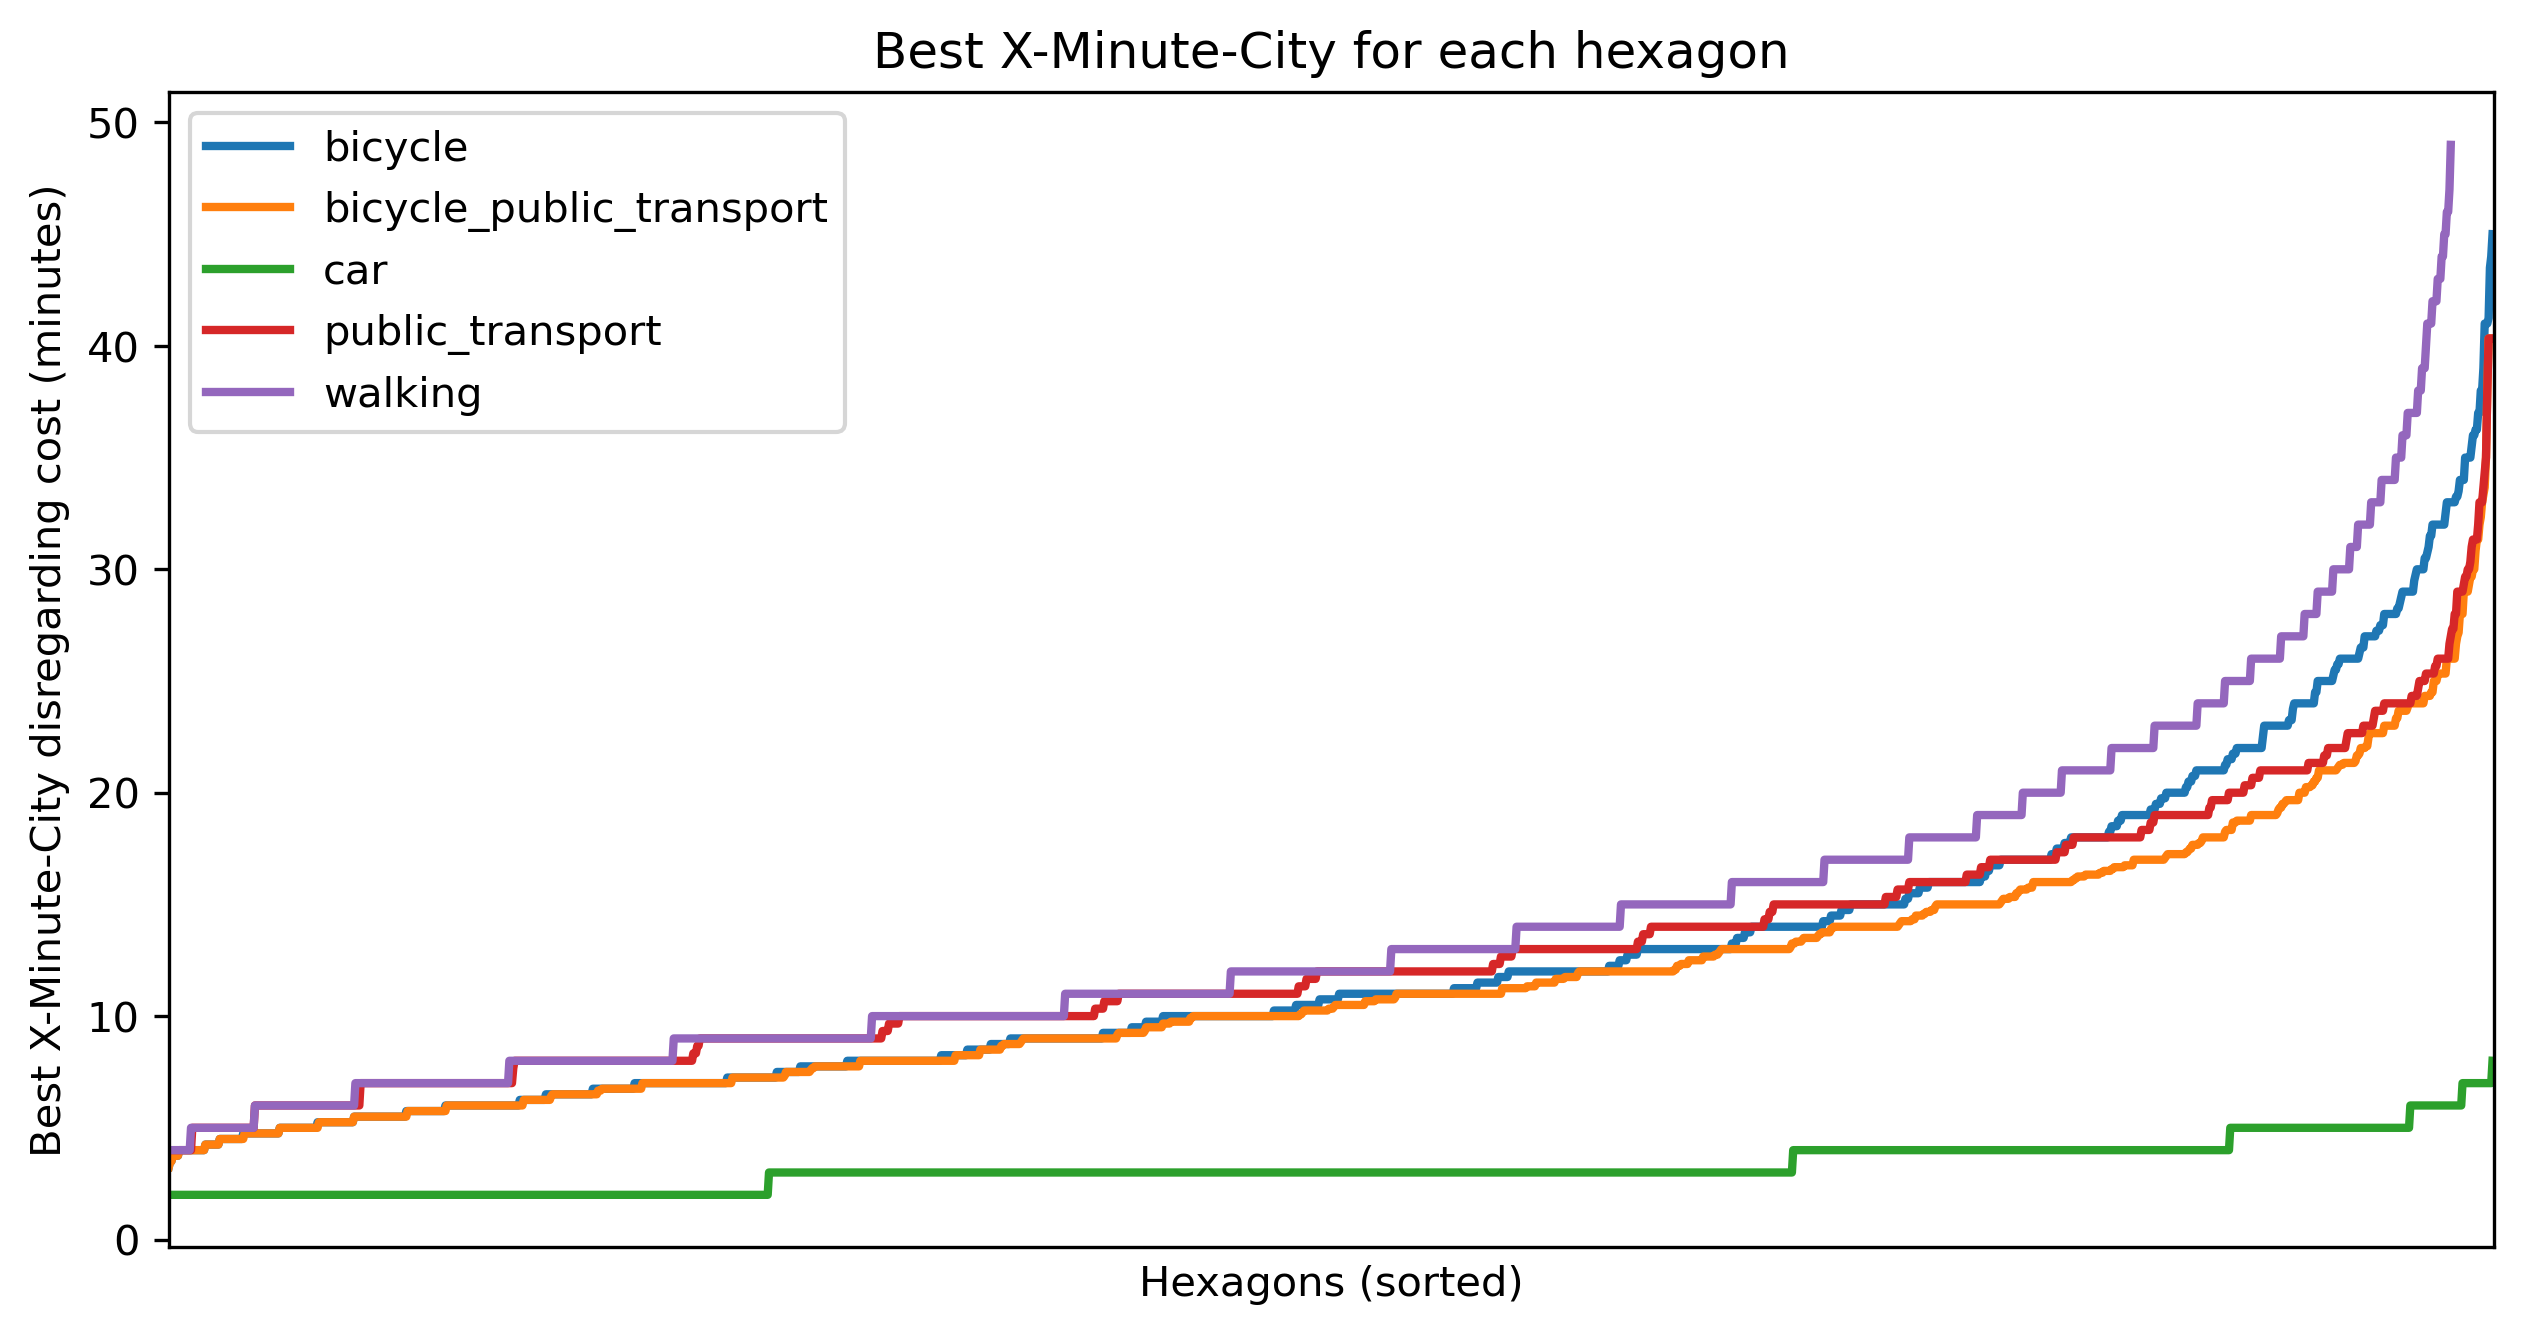
\includegraphics[width=0.85\textwidth]{Figures/results/minute_city_metric/best_x_minute_city}
  \end{center}
  \caption{Distribution of Optimal X-Minute City Metric}
  \label{fig:optimal_x_minute_city_metric}
\end{figure}
As we can see, for the most accessible hexagons to the left, public transport, and walking are the same, but with the less accessible hexagons to the right, public transport becomes better than walking.
In addition, the public transport scenario is worse than the pure bicycle sharing scenario but catches up and even overtakes it as we move to less accessible hexagons.
The same pattern can be observed when comparing the bicycle-sharing scenario to the combined scenario of bicycle-sharing and public transport.
For the most accessible hexagons to the left, the combined scenario is the same as the bicycle-sharing scenario, but as we move to less accessible hexagons to the right, the combined scenario becomes better.
Similarly, when comparing the bicycle-sharing scenario to the combined scenario, we see that the combined scenario provides much better accessibility initially, but as we move to the least accessible hexagons, both become the same.
Generally, adding public transport can slow down the drastic increase of the optimal X-minute city metric at the end of the distribution.


Figure \ref{fig:optimal_map} shows the optimal X-minute city metric for each hexagon over all sustainable modes of travel, i.e., excluding the car scenario.
\begin{figure}
  \begin{center}
    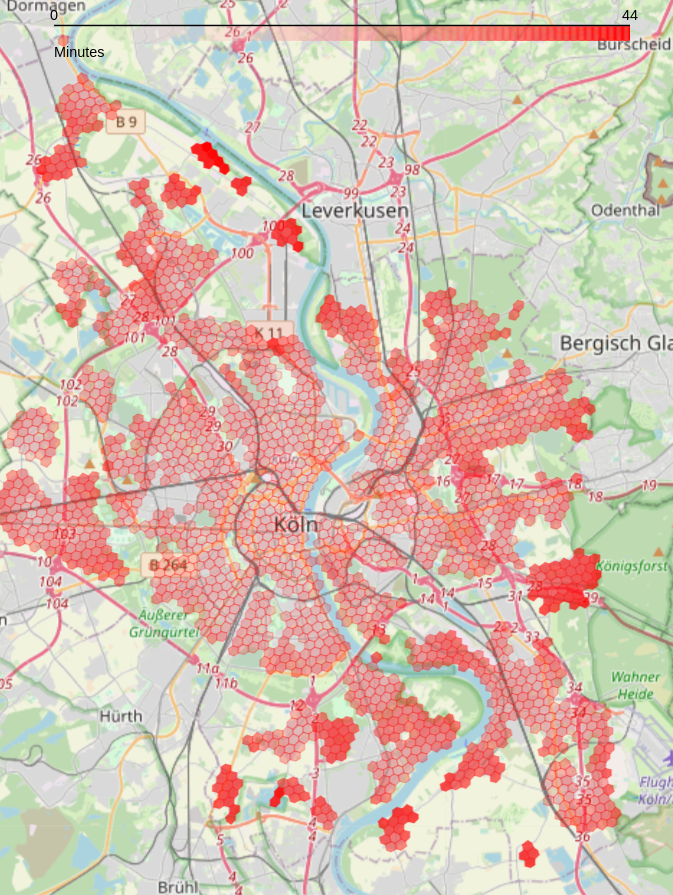
\includegraphics[width=0.45\textwidth]{Figures/results/minute_city_metric/optimal_map}
  \end{center}
  \caption{Map of Optimal X-Minute City Metric}
  \label{fig:optimal_map}
\end{figure}
We can see that the least accessible hexagons require 44 minutes to reach all categories if only sustainable modes of travel are used.
The least accessible regions are suburban areas in the north, south and west of Cologne. 
The region on the left bank of the Rhine River next to Leverkusen, which is the district of Merkenenich, is especially inaccessible.

Figure \ref{fig:optimal_map_per_scenario} shows multiple maps of the optimal X-minute city metric for each hexagon, one for bicycle sharing, one for public transport, and one for walking.
\begin{figure}
     \centering
     \begin{subfigure}[b]{0.3\textwidth}
         \centering
         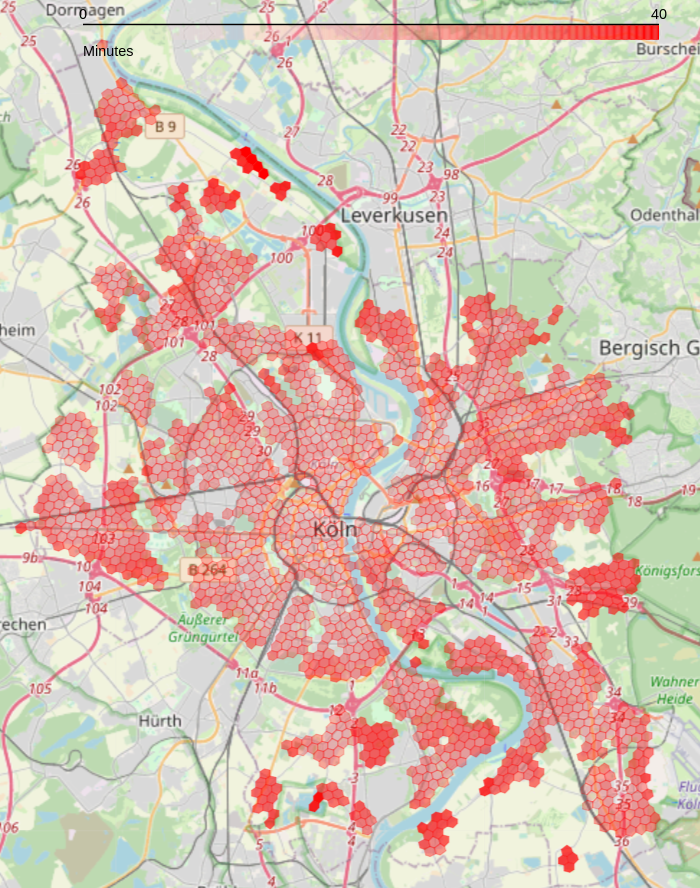
\includegraphics[width=\textwidth]{Figures/results/minute_city_metric/public_transport_optimal_map}
         \caption{Public Transport}
         \label{fig:public_transport_optimal_map}
     \end{subfigure}
     \hfill
     \begin{subfigure}[b]{0.3\textwidth}
         \centering
         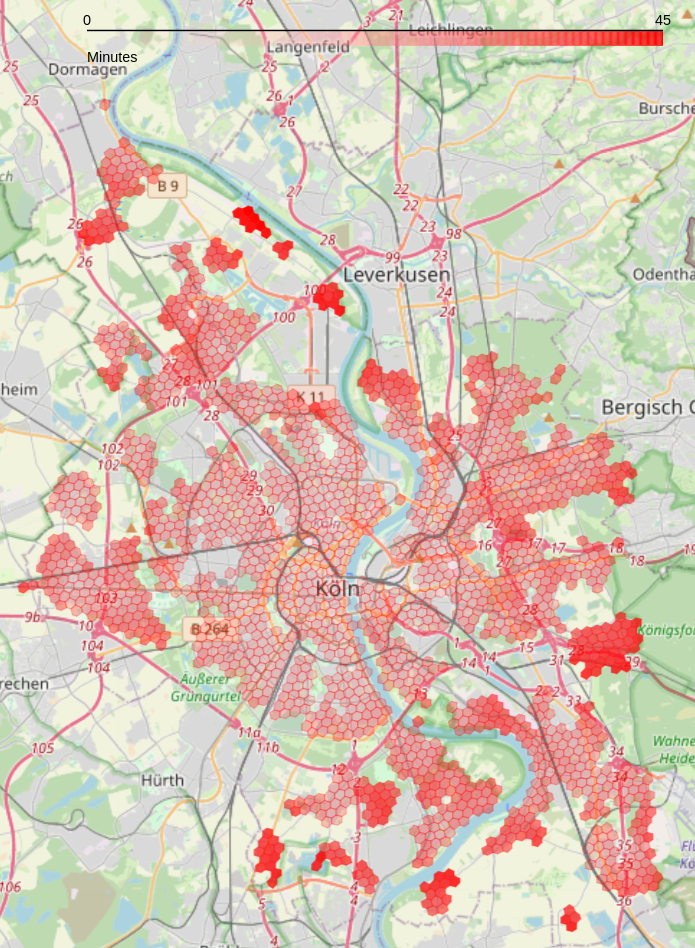
\includegraphics[width=\textwidth]{Figures/results/minute_city_metric/bicycle_optimal_map}
         \caption{Bicycle Sharing}
         \label{fig:bicycle_optimal_map}
     \end{subfigure}
     \hfill
     \begin{subfigure}[b]{0.3\textwidth}
         \centering
         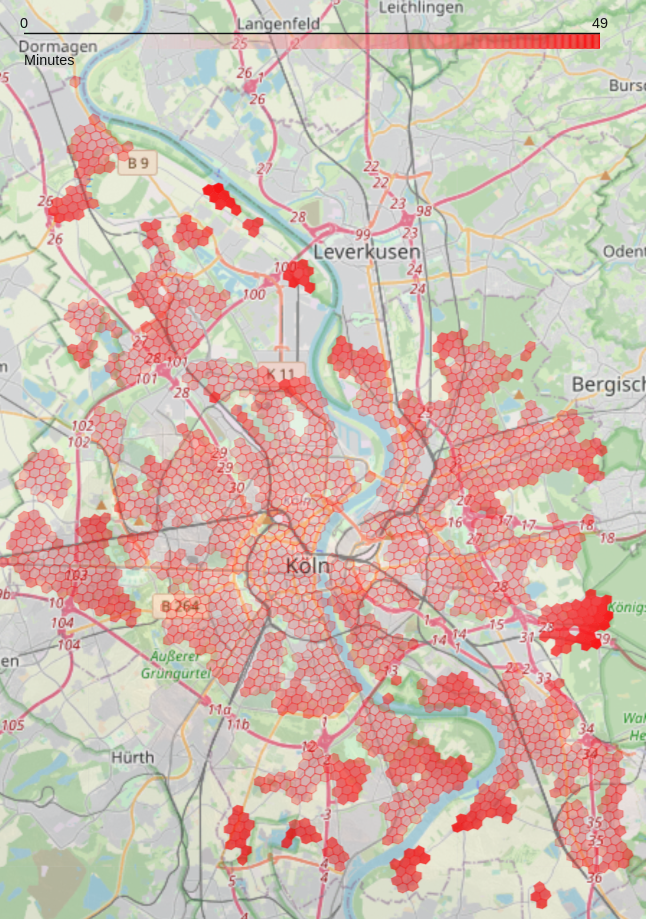
\includegraphics[width=\textwidth]{Figures/results/minute_city_metric/walking_optimal_map}
         \caption{Walking}
         \label{fig:walking_optimal_map}
     \end{subfigure}
        \caption{Map of Optimal X-Minute City Metric per Scenario}
        \label{fig:optimal_map_per_scenario}
\end{figure}
The areas in and around the city center are more accessible by bicycle sharing than by public transport and walking.
In the east of the city, near the forest "Königsforst", we see the district of Rath/Neumar, with low accessibility for all scenarios.
However, one can see that the region is more accessible by public transport than by bicycle sharing and walking.

\subsection{Cost}
\label{subsec:cost_of_15_minute_city}

% table (mean, quantiles) of required cost
Table \ref{tab:required_cost} shows the mean, the 25\%, 50\%, and 75\% quantiles and the maximum of the costs that are required to achieve the optimal value for the X-minute city shown in Section \ref{subsec:15_minute_city_metric}.
\begin{table}
  \caption{Required Cost for Optimal Over All Hexagons}
  \label{tab:required_cost}
  \begin{center}
    \begin{tabular}{lrrrrr}
     & mean & 25\% & 50\% & 75\% & max \\
    scenario &  &  &  &  &  \\
    Bicycle & 0.39 & 0.00 & 0.50 & 0.75 & 1.00 \\
    Car & 0.36 & 0.19 & 0.38 & 0.38 & 1.14 \\
    Combined & 0.86 & 0.00 & 0.75 & 1.30 & 3.95 \\
    Public Transport & 0.64 & 0.00 & 0.00 & 1.47 & 3.20 \\
    Walking & 0.00 & 0.00 & 0.00 & 0.00 & 0.00 \\
    \end{tabular}
  \end{center}
\end{table}
We can immediately see that there is no cost for hexagons at the 25\% and 50\% quantile when using public transport, implying that public transport is not used at all for those hexagons.
Looking at the 75\% quantile and the maximum required cost for an optimal X-Minute City metric for public transport, we see that the benefits we observed earlier come at a cost.
Similarly, bicycle sharing and the combined mode have zero cost at the 25\% quantile, implying that they are not used for those hexagons.

Looking at the maximum cost values of each sustainable mode of transport shows us that bicycles never require more than \euro{1}.
As \euro{1} allows to travel a maximum of 15 minutes, it is never necessary to travel longer than 15 minutes after a bicycle is reached.
The maximum cost incurred by public transport is \euro{3.20}, the long-distance ticket of public transport (more than four stops) is used.
Similarly, in the combined scenario, the long-distance ticket is used with a 15-minute ride of bicycle sharing in at least one sub-scenario, resulting in the maximum price of \euro{3.95}.
Remember that the values we observer are average values of all sub-scenarios belong to a scenario.
Because of this the maximum price is \euro{3.95} and not \euro{4.20} (\euro{1} + \euro{3.20}), as not all sub-scenarios reach the maximum of \euro{4.20}.

We can make similar observations with more granularity when looking at the distribution of the required cost in Figure \ref{fig:maximum_required_cost_for_x_minute_city}.
\begin{figure}
  \begin{center}
    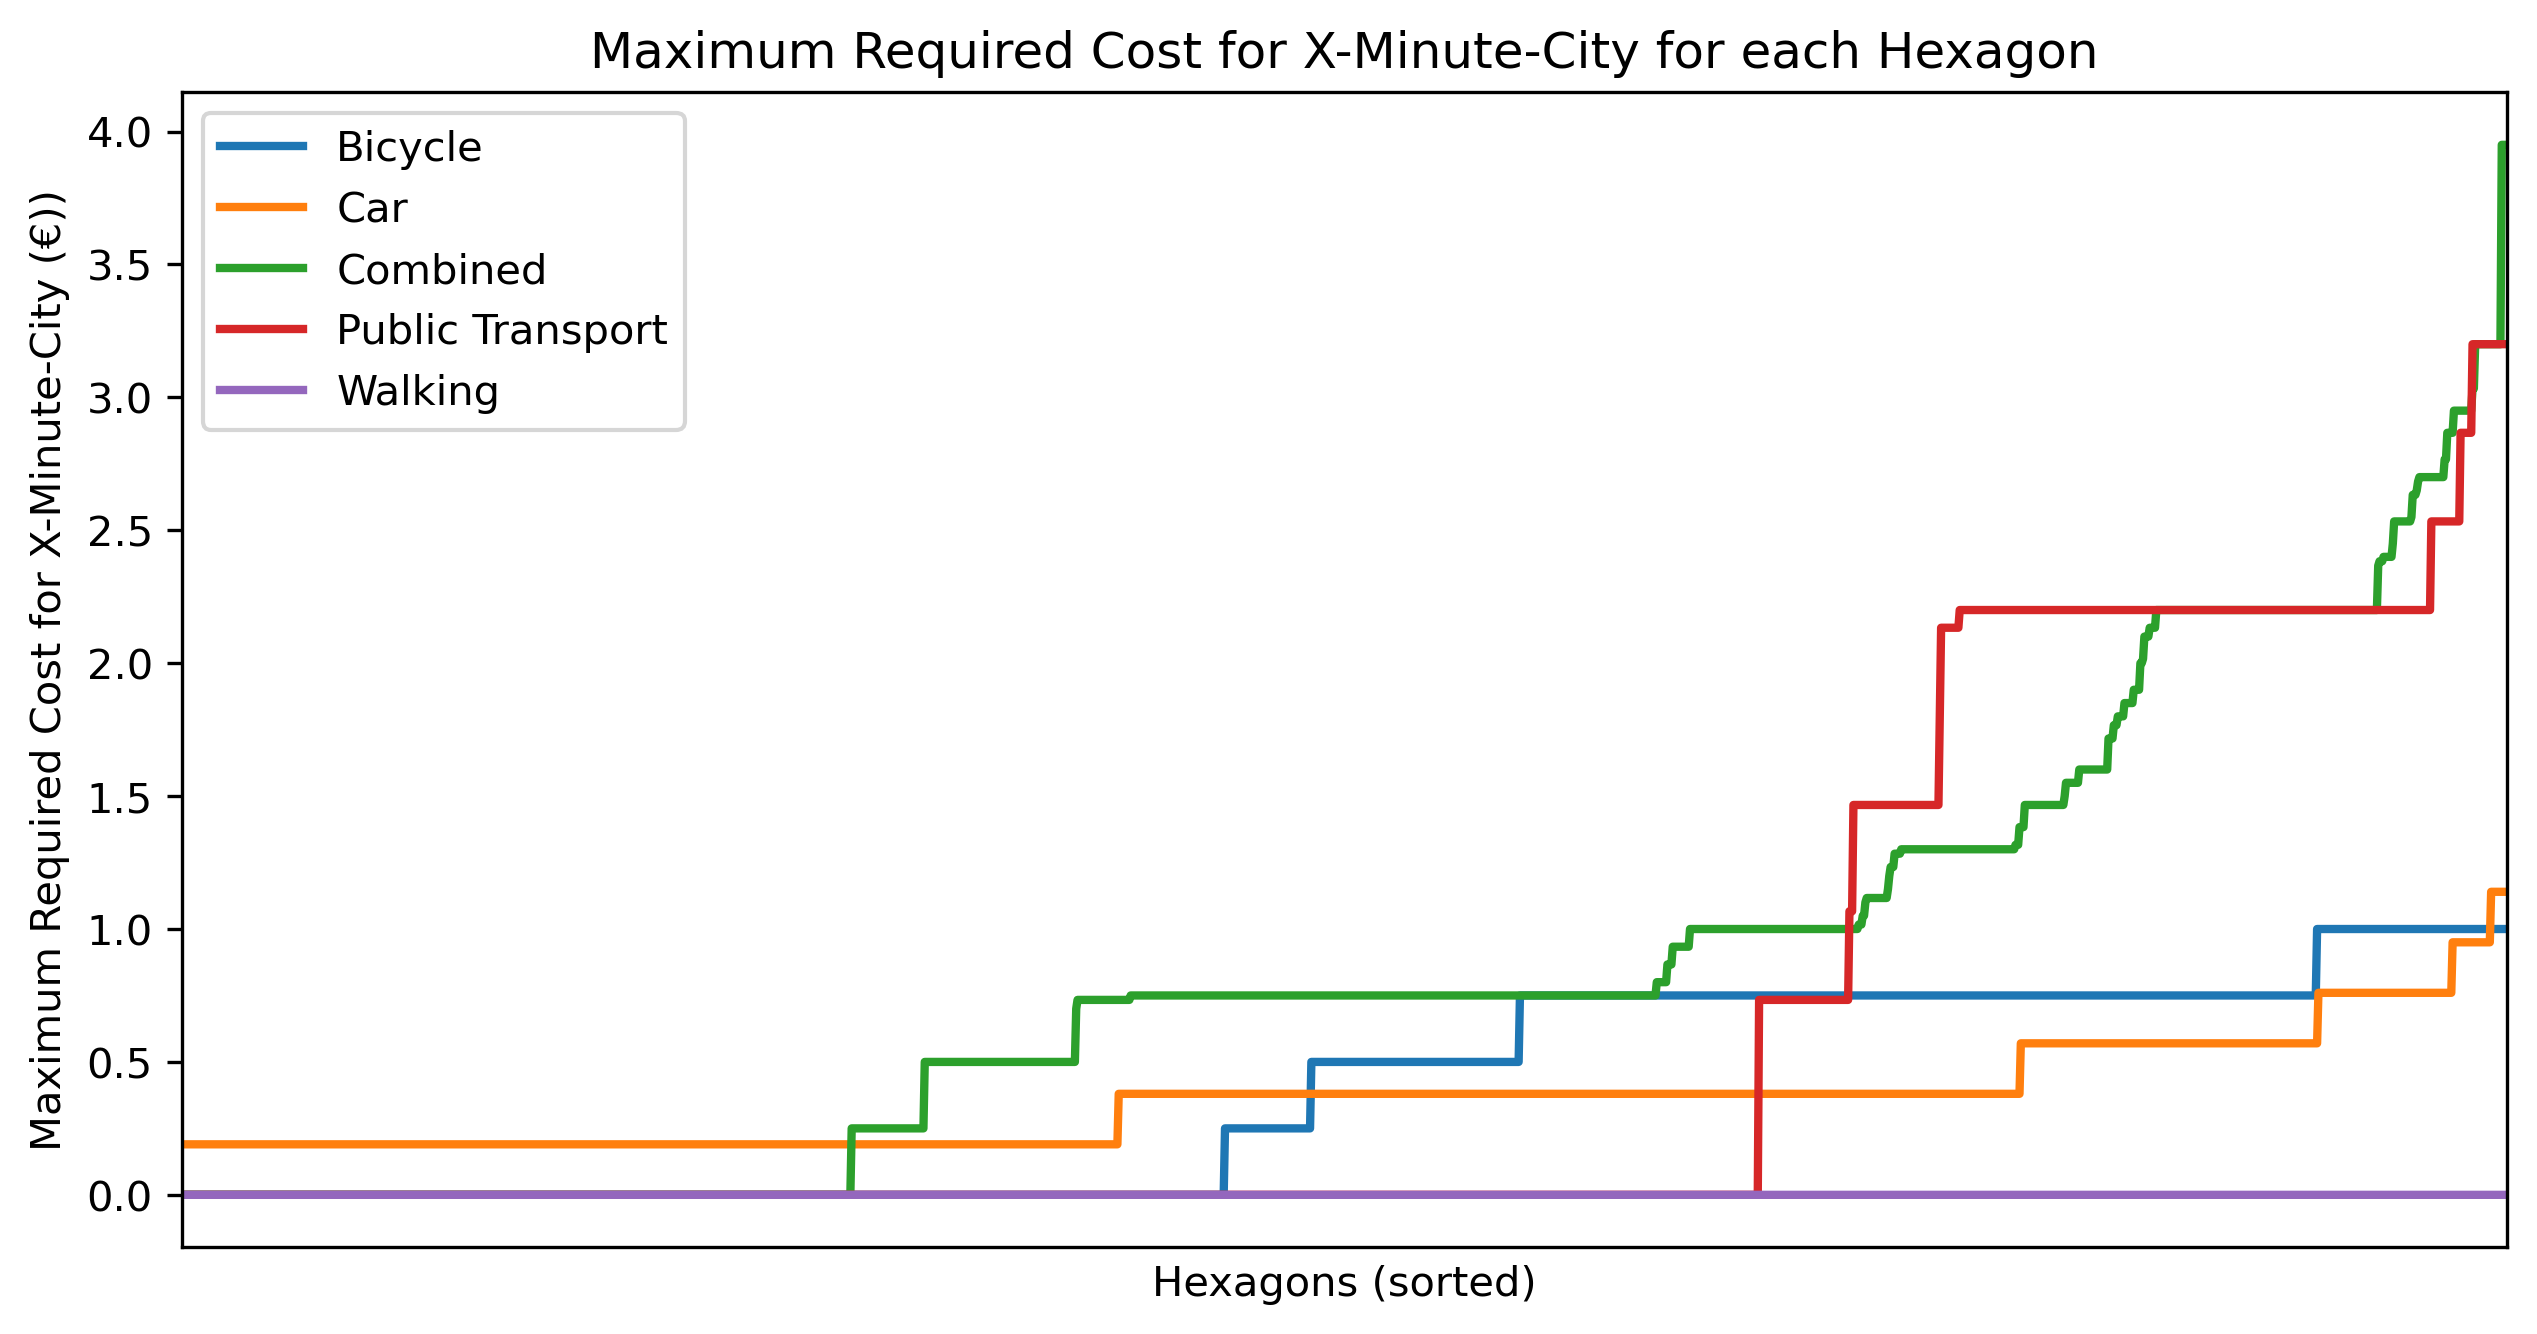
\includegraphics[width=0.65\textwidth]{Figures/results/cost/maximum_required_cost_for_x_minute_city}
  \end{center}
  \caption{Maximum Required Cost for Optimal X-Minute City Metric}
  \label{fig:maximum_required_cost_for_x_minute_city}
\end{figure}
A new pattern stands out when comparing public transport and the combined mode.
We see that the combined mode has higher costs earlier, surpassed by public transport, only to be surpassed again by the combined mode.
% discussion stuff (not sure where to put this)
%The first price increase in the combined mode can be explained by the \euro{1} cost of 15-minute bicycle sharing.
%Then public transport's costs surpassed those of the combined mode the combined mode. 
%This is probably because bicycle sharing is more cost-efficient and can somewhat replace public transport.
%The fact that the combined mode then surpasses public transport again most likely stems from the fact that the combined mode can achieve faster access than public transport by using bicycle sharing, which is more expensive than a short-distance ticket alone.
% END

Figure \ref{fig:cost_map_per_scenario} shows the cost required to reach the optimal X-minute city metric for each hexagon for public transport, bicycle sharing, and the combined scenario of bicycle sharing and public transport.
Note that we do not show the cost for the walking scenario, as it is always \euro{0}.
In these figures, we see that sometimes the cost is zero.
As the portrayed scenarios all have costs associated with them, a cost of zero means that only walking is used.
\begin{figure}
     \centering
     \begin{subfigure}[b]{0.3\textwidth}
         \centering
         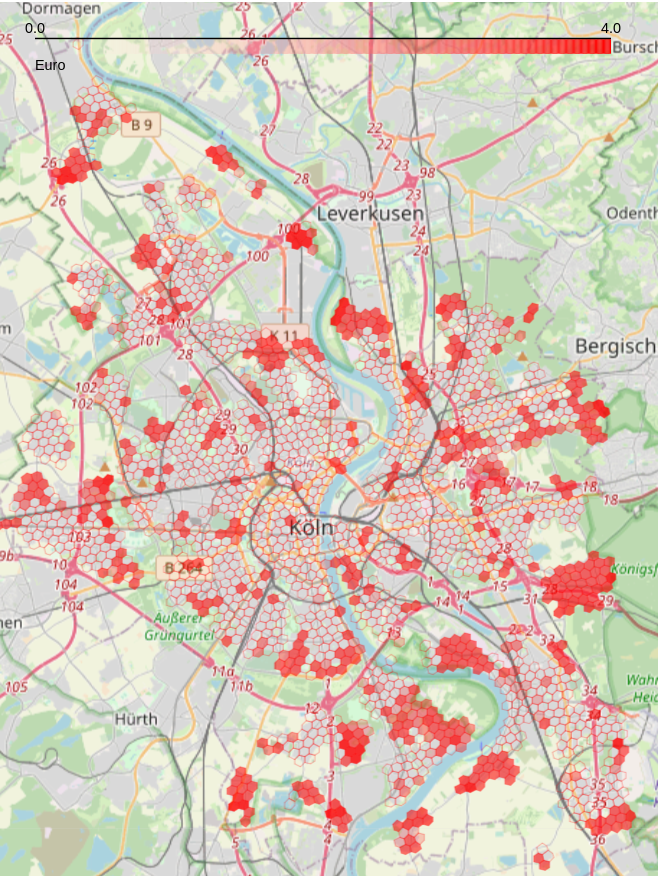
\includegraphics[width=\textwidth]{Figures/results/cost/public_transport_cost_map}
         \caption{Public Transport}
         \label{fig:public_transport_cost_map}
     \end{subfigure}
     \hfill
     \begin{subfigure}[b]{0.3\textwidth}
         \centering
         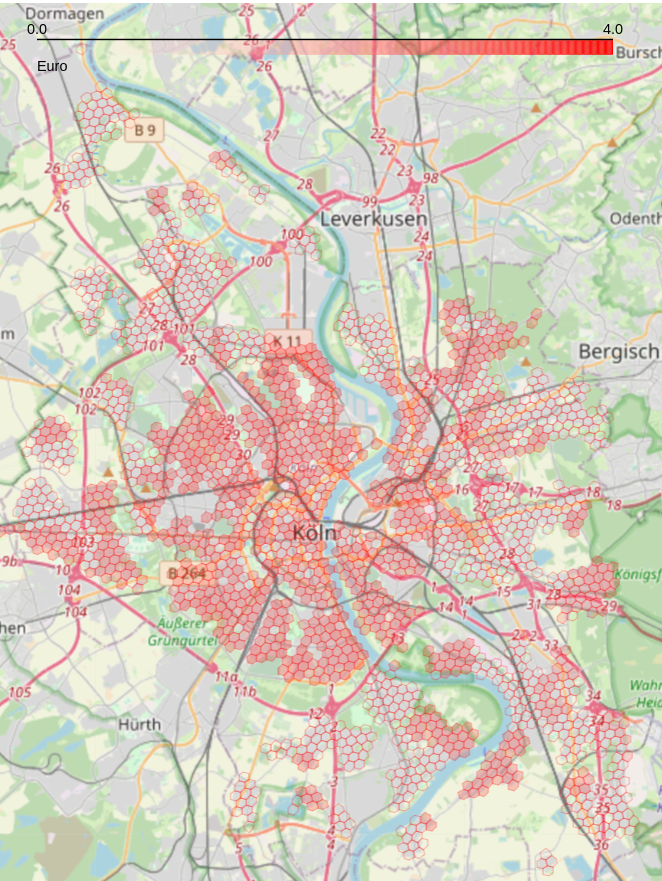
\includegraphics[width=\textwidth]{Figures/results/cost/bicycle_cost_map}
         \caption{Bicycle Sharing}
         \label{fig:bicycle_cost_map}
     \end{subfigure}
     \hfill
     \begin{subfigure}[b]{0.3\textwidth}
         \centering
         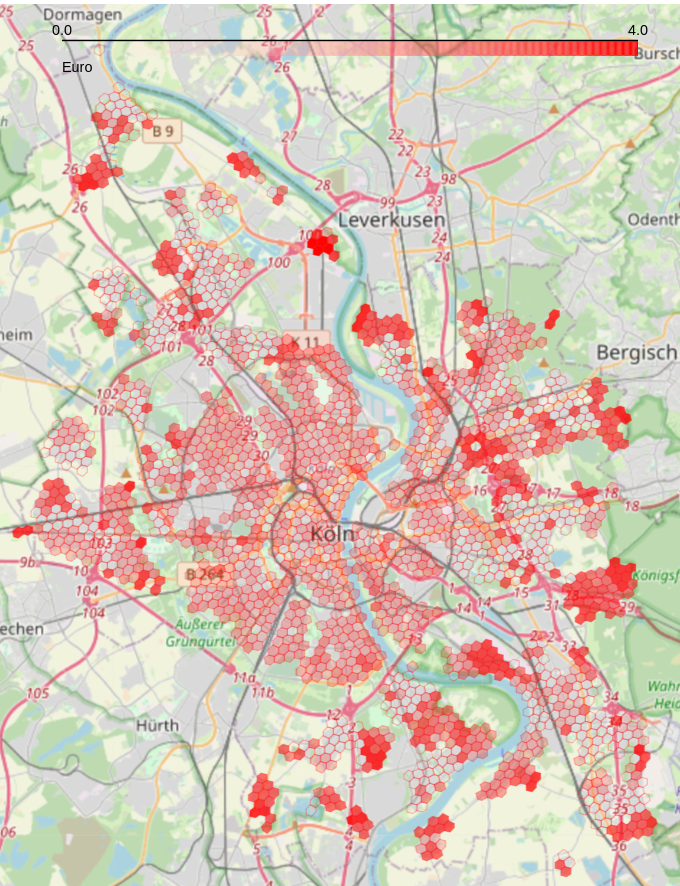
\includegraphics[width=\textwidth]{Figures/results/cost/bicycle_public_transport_cost_map}
         \caption{Combined}
         \label{fig:bicycle_public_transport_cost_map}
     \end{subfigure}
       \caption{Map of Required Cost for Optimal for Each Hexagon}
        \label{fig:cost_map_per_scenario}
\end{figure}
We see almost in all hexagons in and around the city center, where NextBike's flex zone is located, the cost for the bicycle sharing scenario is \euro{1}.
This sometimes also extends outside the city center.
The cost of public transport is more scattered around the whole region. 
We can mostly see single hexagons in the city's center and small groups of hexagons outside the city that have costs higher than zero.
For the combined mode we see a pattern that roughly is equal to the union of the public transport and bicycle sharing scenario.

\subsection{Interaction Between Cost and X-Minute City Metric}
\label{subsec:interaction_between_cost_and_15_minute_city_metric}

Next, we will examine the interaction between the cost and the optimal X-minute city metric.
To do so, we will investigate the mean Pareto front of the X-minute city metric and cost over all hexagons.
Before performing the analysis for the whole region of Cologne, we first examine the Pareto front of a single hexagon, which is depicted in Figure \ref{fig:example_pareto_front}.
The x-axis shows the cost, and the y-axis shows the X-minute city metric.
The line shows us what X-minute city metric is achievable for a given cost in a specific scenario.

\begin{figure}
  \begin{center}
     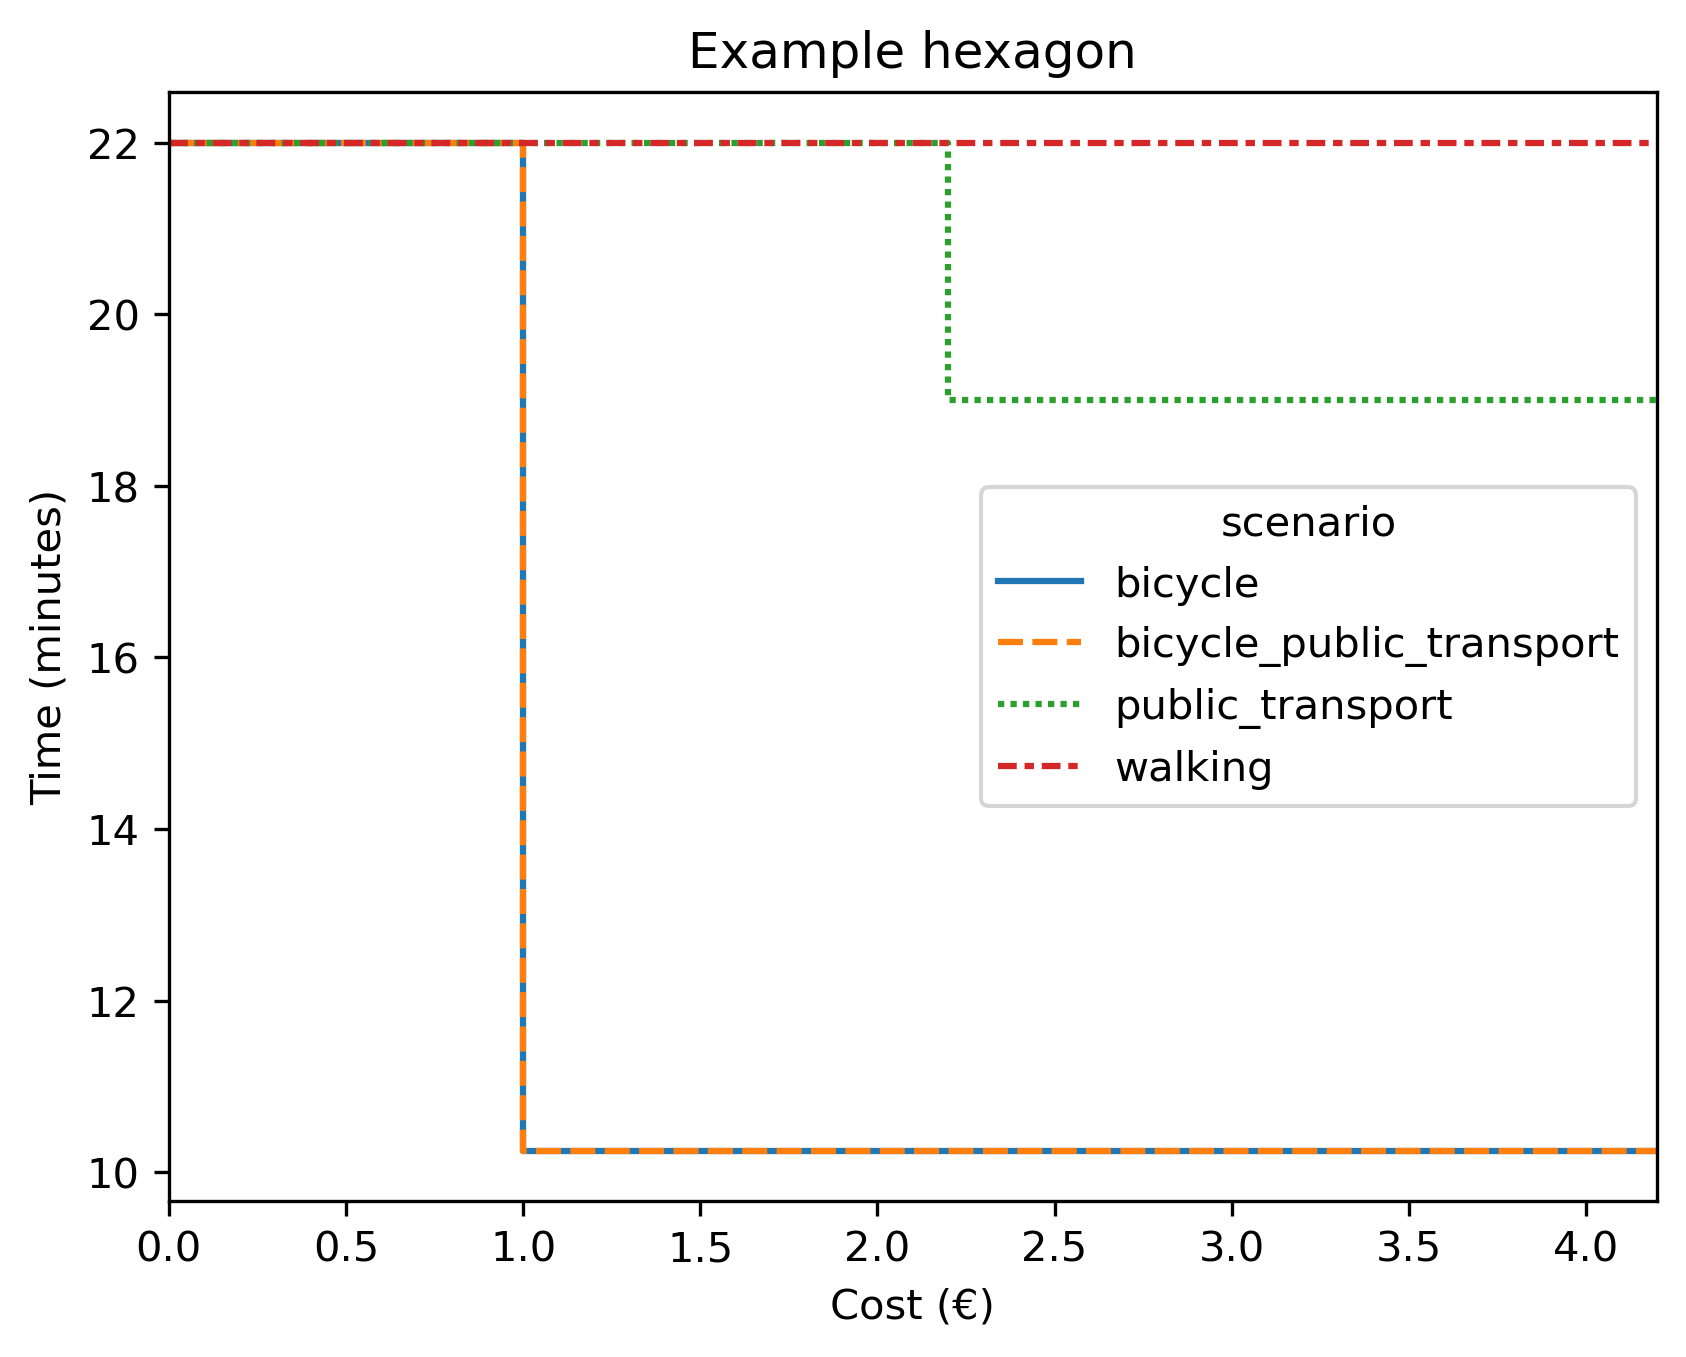
\includegraphics[width=0.5\textwidth]{Figures/results/metric_cost/example_profile}
  \end{center}
  \caption{Example Pareto Front}
  \label{fig:example_pareto_front}
\end{figure}

In our example, all modes begin with an accessibility value of 22 minutes for a cost of \euro{0}.
Increasing the cost only yields improvements when reaching a cost of \euro{1}, where the bicycle and combined scenarios can reach all categories within approximately 10 minutes.
Further, increasing the price to \euro{2.20} improves the public transport scenario, where reaching all categories within approximately 19 minutes is now possible.
Further cost increases do not yield any improvements for any scenario.

We can also quantify the value of the improvements as seen in Table \ref{tab:differences_in_example_hexagon}.
This table shows all the steps visible in the previous graph with their cost and magnitude of improvement.
In addition, we can calculate the benefit in minutes per one euro of cost to make the value of the steps more comparable.
\begin{table}
  \caption{Steps in Example hexagon}
  \label{tab:differences_in_example_hexagon}
  \begin{center}
    \begin{tabular}{lrrrl}
     scenario & Improvement & At cost (\euro) & Improvement (min/\euro) \\
     Bicycle & 11m 45s & 1.00 & 11.75 \\
     Combined & 11m 45s & 1.00 & 11.75 \\
     Public Transport & 3m 00s & 2.20 & 1.36 \\
    \end{tabular}
  \end{center}
\end{table}
As we can see, the bicycle scenarios' increase at a cost of \euro{1} is larger than the public transport scenario's increase and has a higher value per euro.

% generalization
To generalize these findings over all hexagons, we take the average over the X-minute city for each cost and scenario to generate an average Pareto front.
The resulting Pareto front can be seen in Figure \ref{fig:mean_time_per_cost}.
\begin{figure}
  \begin{center}
     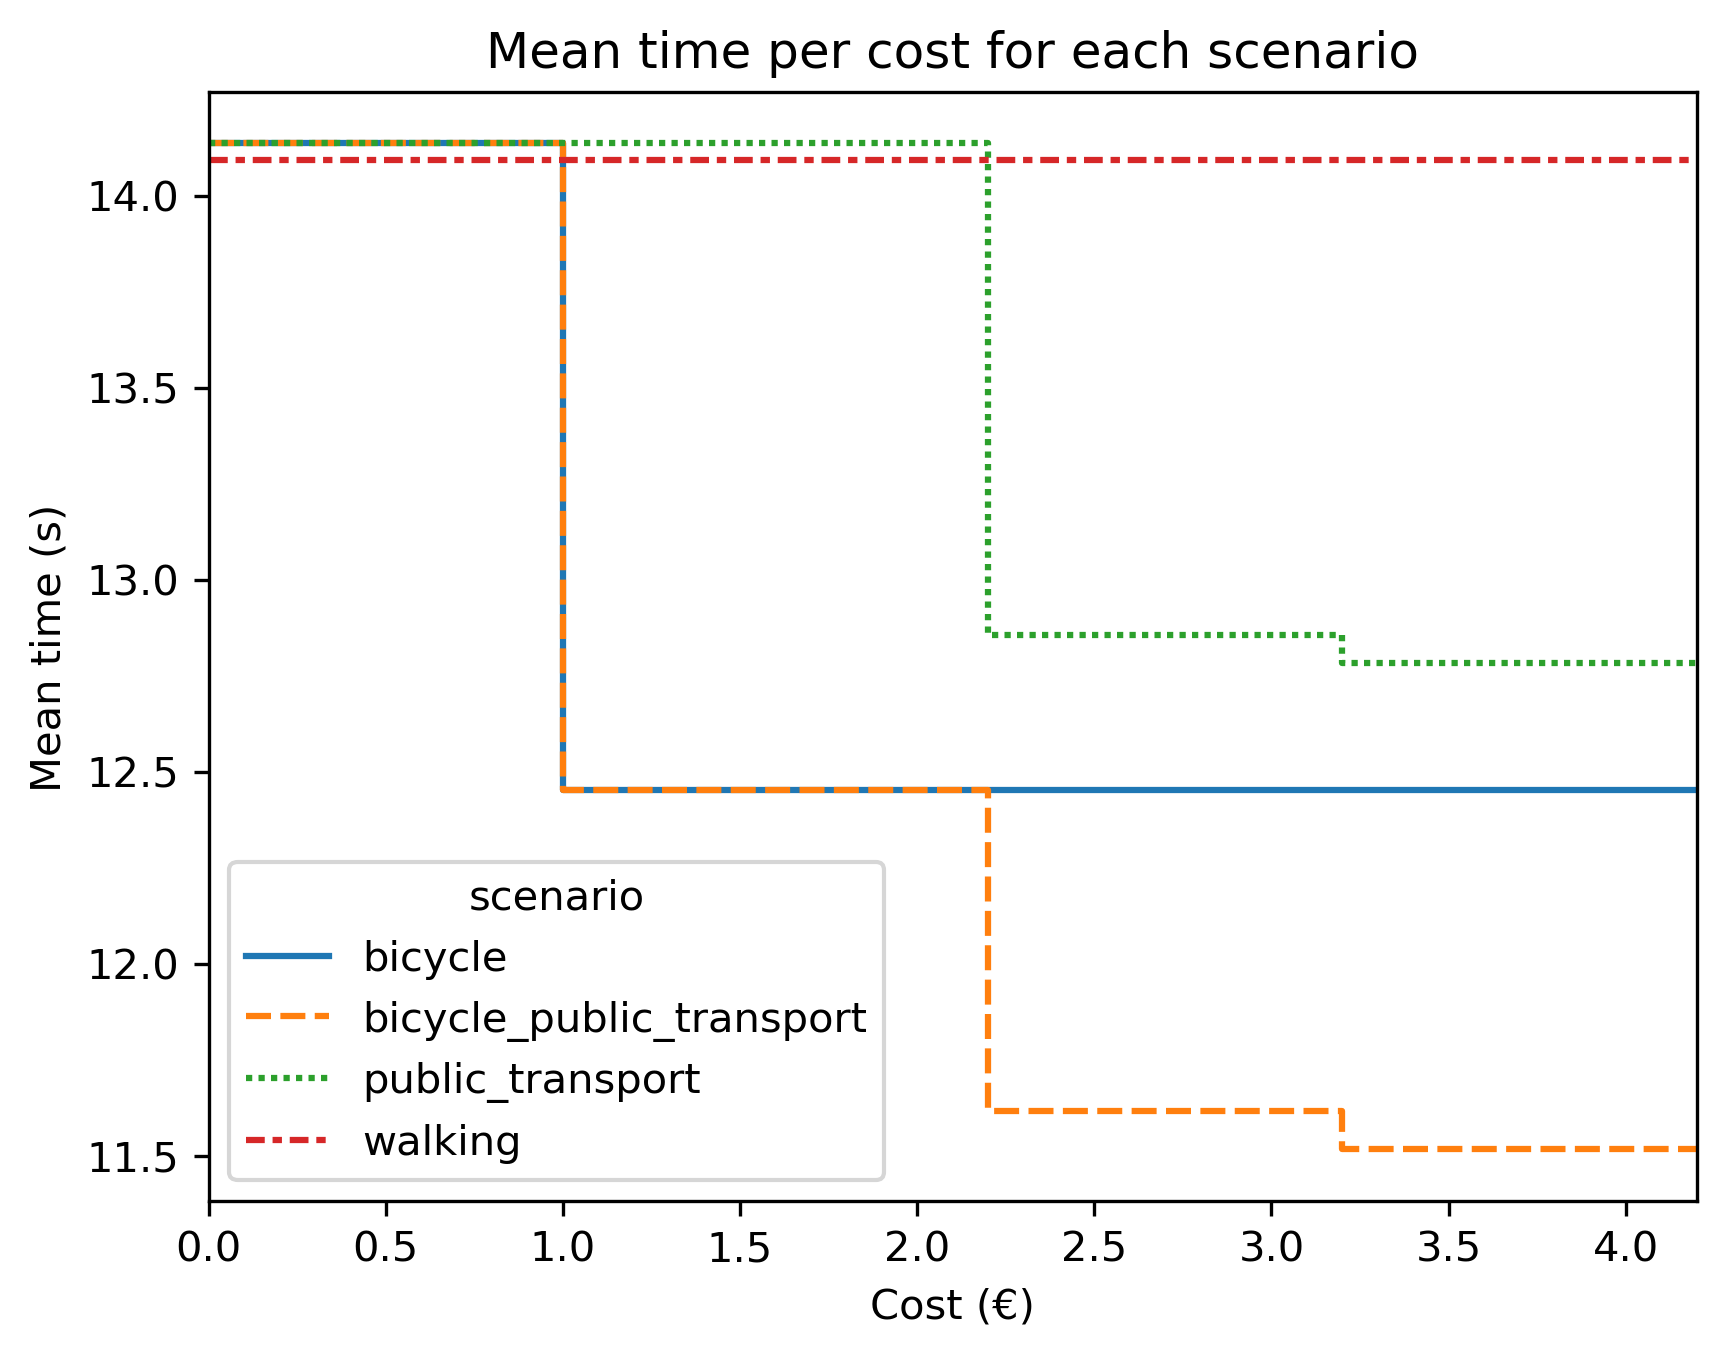
\includegraphics[width=0.5\textwidth]{Figures/results/metric_cost/mean_time_per_cost}
  \end{center}
  \caption{Mean Time per Cost for All Scenarios}
  \label{fig:mean_time_per_cost}
\end{figure}
Similarly to the example of the single hexagon from before, we can see improvements for the bicycle scenario and the combined scenario at the cost of \euro{1} of about 1 minute and 30 seconds.
We can also see the improvements in public transport at a cost of \euro{2.20}.
Unlike in the example of the single hexagon, we can also see the improvement at the cost of \euro{2.20} for the combined scenario.
Lastly, there is a slight improvement for the public transport scenario and the combined scenario at a cost of \euro{3.20}.

To compare these improvements, we can again look at the differences in Table \ref{tab:differences_in_mean_pareto_front}.
We won't analyze the differences in the combined scenario, as prior improvements of other modes skew the improvements, which results in numbers that are hard to interpret.

\begin{table}
  \caption{Steps in Mean Pareto Front}
  \label{tab:differences_in_mean_pareto_front}
  \begin{center}
    \begin{tabular}{lrrrrl}
     Scenario & Improvement & At cost (\euro) & Cost diff (\euro) & Improvement (min/\euro) \\
     Bicycle & 1m 41s & 1.00 & 1.00 & 1.684 \\
     Public transport & 1m 16s & 2.20 & 2.20 & 0.583 \\
     Public transport & 0m 04s & 3.20 & 1.00 & 0.074 \\
    \end{tabular}
  \end{center}
\end{table}

We see that the improvements of the bicycle scenario at the cost of \euro{1} are the largest, with an improvement of 1 minute and 41 seconds, and also the most cost-effective, with a value of 1.68 minutes per euro.
They are followed by the improvements of the public transport scenario at a cost of \euro{2.20} with an improvement of 1 minute and 16 seconds and a value of 0.58 minutes per euro.
The improvement at a cost of \euro{3.20} is minimal and the least cost-effective.

Next, we are going to look at the quantiles of the aggregated Pareto front.
Figure \ref{fig:quantile_time_per_cost} shows the 25\%, 75\%, and 90\% quantiles of the aggregated Pareto front.
The 25\% quantile gives us insights about the more accessible areas in the city.
Note that because we aggregate all the values of the X-minute city metric for a single cost and scenario at a time, the 25\% quantile Pareto front does not necessarily reflect the same 25\% of hexagons for each cost.

\begin{figure}
     \centering
     \begin{subfigure}[b]{0.48\textwidth}
         \centering
         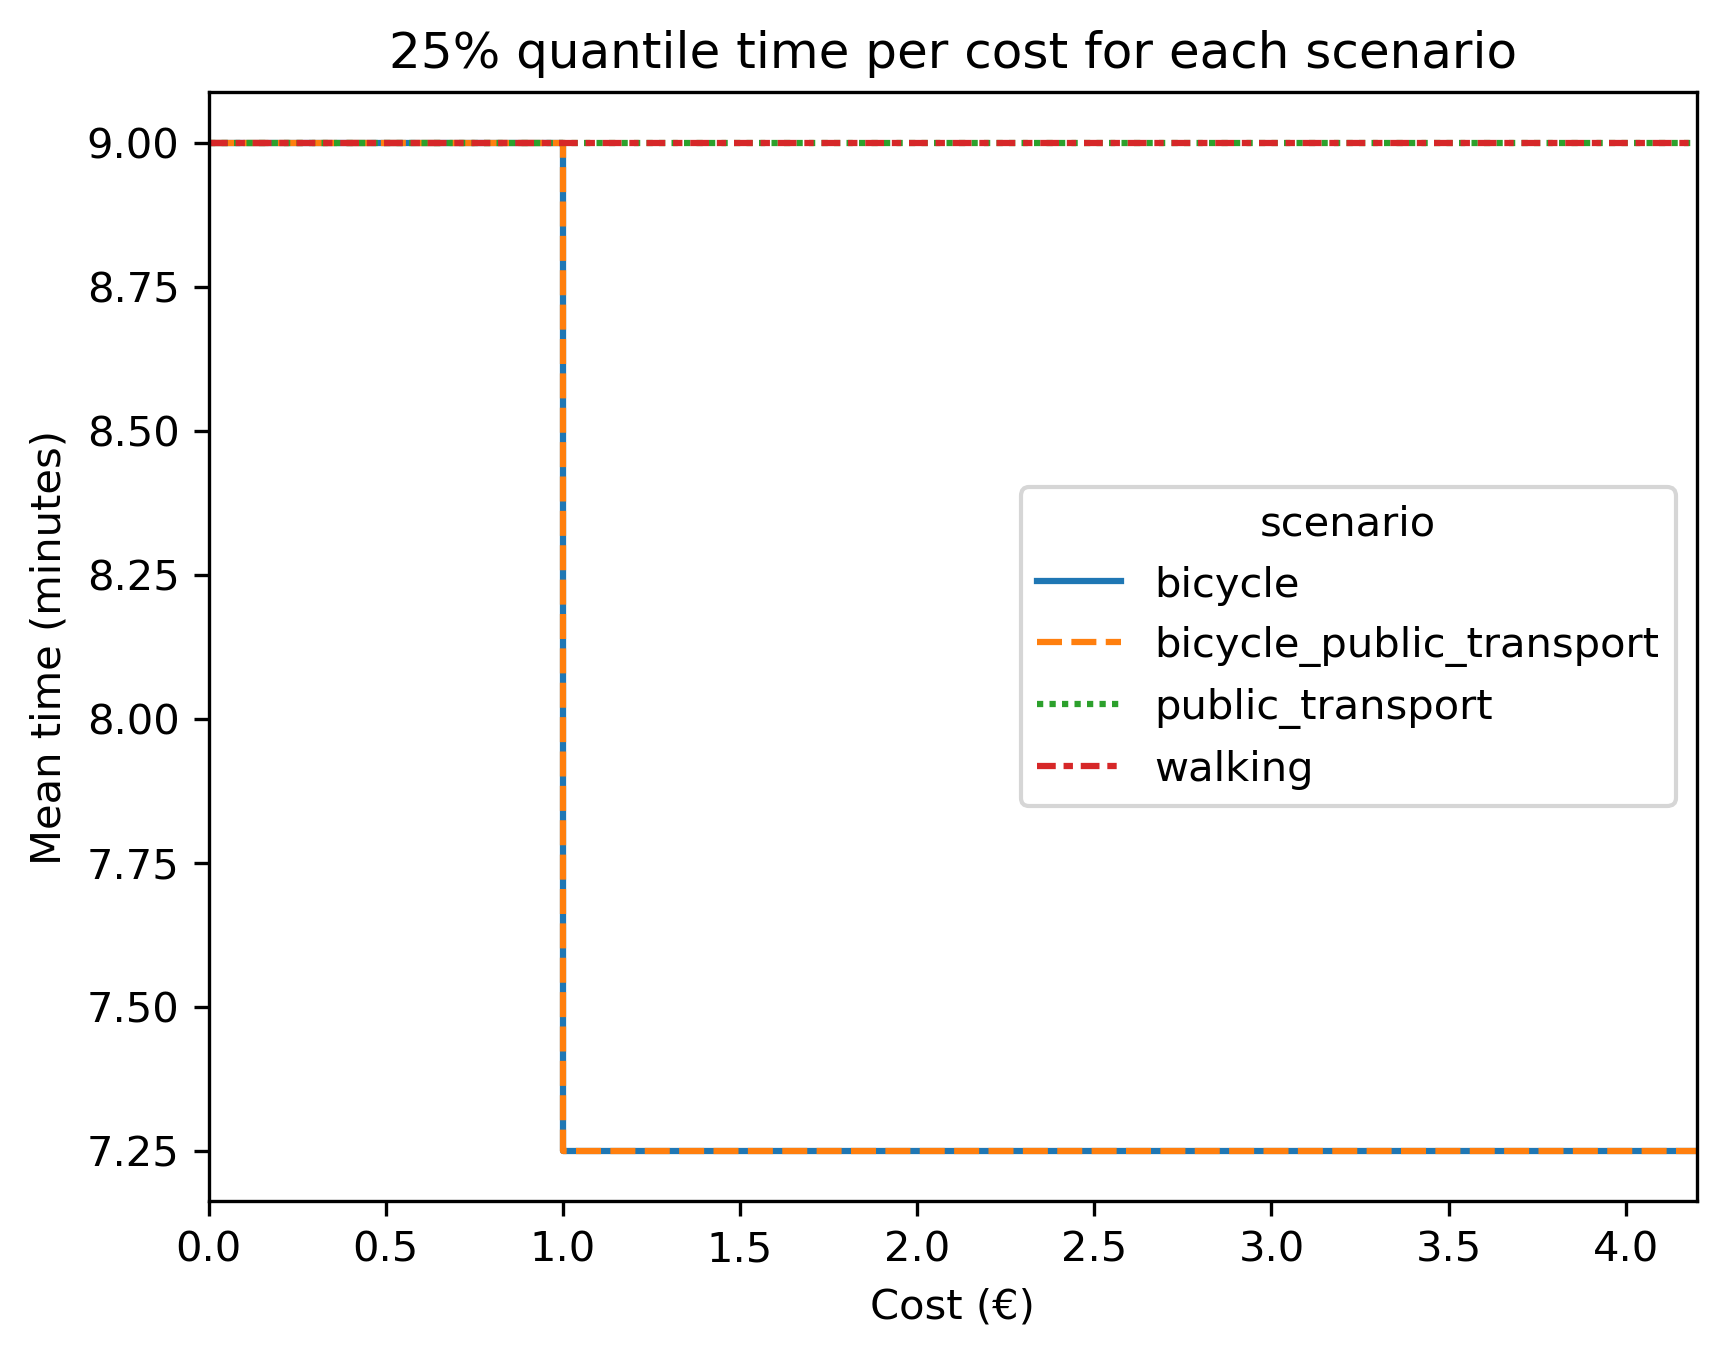
\includegraphics[width=\textwidth]{Figures/results/metric_cost/quantile_25_time_per_cost_for_each_scenario_without_car.png}
         \caption{25\% quantile time per cost for all scenarios}
         \label{fig:25_quantile_time_per_cost}
     \end{subfigure}
     \hfill
     \begin{subfigure}[b]{0.48\textwidth}
         \centering
         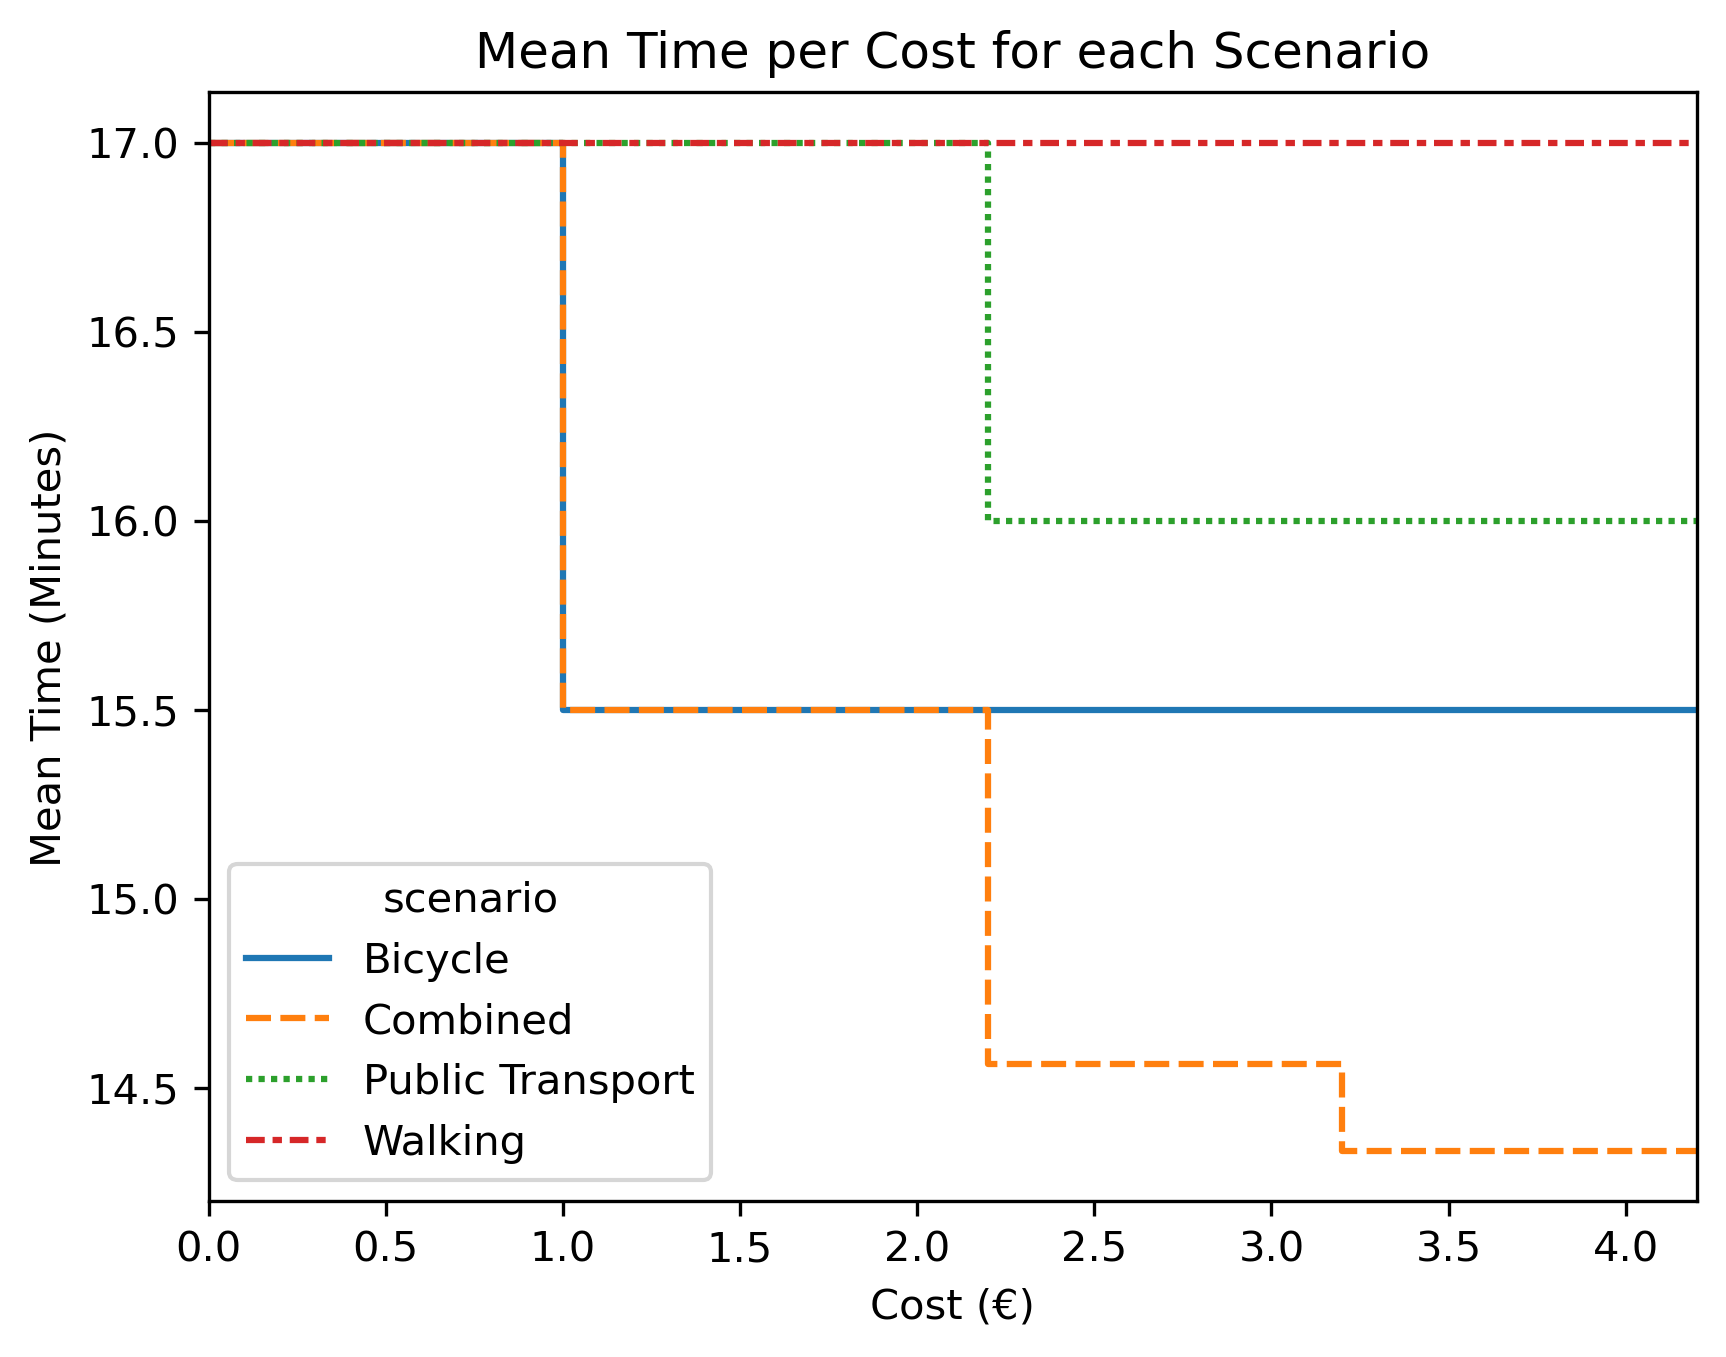
\includegraphics[width=\textwidth]{Figures/results/metric_cost/quantile_75_time_per_cost_for_each_scenario_without_car.png}
         \caption{75\% quantile time per cost for all scenarios}
         \label{fig:75_quantile_time_per_cost}
     \end{subfigure}
     \hfill
     \begin{subfigure}[b]{0.48\textwidth}
         \centering
         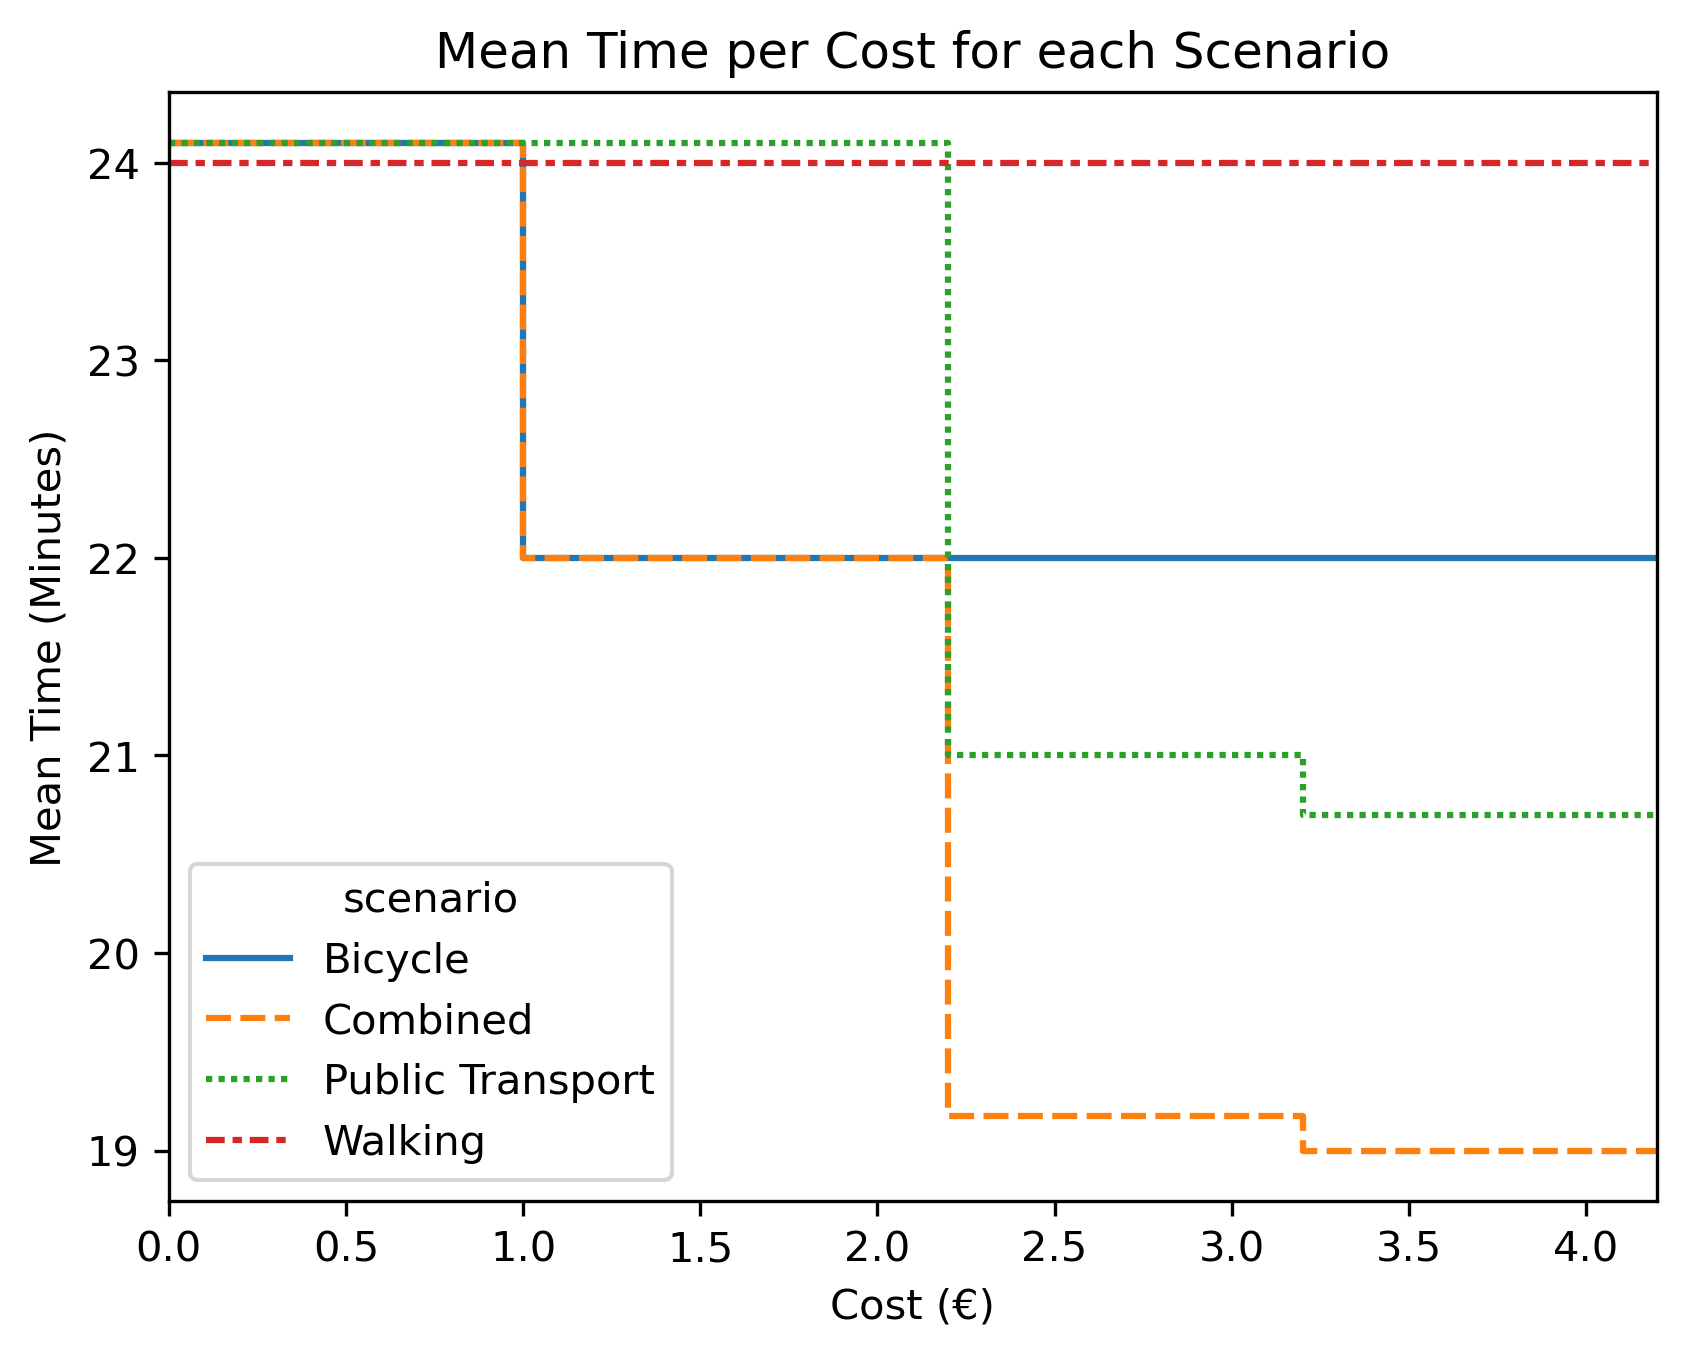
\includegraphics[width=\textwidth]{Figures/results/metric_cost/quantile_90_time_per_cost_for_each_scenario_without_car.png}
         \caption{90\% quantile time per cost for all scenarios}
         \label{fig:90_quantile_time_per_cost}
     \end{subfigure}
        \caption{Map of Optimal X-minute City Metric per Scenario}
        \label{fig:quantile_time_per_cost}
\end{figure}
The 25\% quantile Pareto front shown in Figure \ref{fig:25_quantile_time_per_cost} only contains a single improvement at the cost of \euro{1} for scenarios containing bicycle sharing of 1 minute and 45 seconds with a cost-effectiveness of 1.75 minutes per euro.
The 75\% quantile Pareto front shown in Figure \ref{fig:75_quantile_time_per_cost} with its steps shown in Table \ref{tab:differences_in_75_quantile_pareto_front} also has a similar improvement of 1 minute and 30 seconds at the cost of \euro{1} for bicycle scenarios.
In addition to that, it also shows a smaller increase at \euro{2.20} of 1 minute and an even smaller increase at \euro{3.20} for the public transport and combined scenarios.
\begin{table}
  \caption{Steps in 75\% Quantile Pareto Front}
  \label{tab:differences_in_75_quantile_pareto_front}
  \begin{center}
    \begin{tabular}{lrrrrl}
     Scenario & Improv. & At cost (\euro) & Cost diff (\euro) & Improv. (min/\euro) \\
     Bicycle & 1m 30s & 1.00 & 1.00 & 1.500 \\
     Public transport & 1m 00s & 2.00 & 2.20 & 0.455 \\
    \end{tabular}
  \end{center}
\end{table}
The 90\% quantile Pareto Front shown in Figure \ref{fig:90_quantile_time_per_cost} with its steps shown in Table \ref{tab:differences_in_90_quantile_pareto_front} shows a similar pattern to the 75\% quantile Pareto front.
The significant difference is that the increase at \euro{2.20} for public transport scenarios is larger than the increase at 1 euro for bicycle scenarios.
More precisely, while bicycle sharing is more effective in decreasing the 15-minute city metric on average and for the 75\% most accessible regions, public transport is more effective than bicycle sharing for the 10\% least accessible areas.
In contrast to the other quantiles we examined the improvement of the public transport scenario is larger than that of bicycle sharing. 
However, it is still less cost-effective than the improvement in the bicycle-sharing scenario.


\begin{table}
  \caption{Steps in 90\% Quantile Pareto Front}
  \label{tab:differences_in_90_quantile_pareto_front}
  \begin{center}
    \begin{tabular}{lrrrrl}
     improvement & at cost & cost diff & minute per euro & scenario \\
     3.000 & 2.200 & 2.200 & 1.364 & public transport \\
     2.000 & 1.000 & 1.000 & 2.000 & bicycle \\
     0.033 & 3.200 & 1.000 & 0.033 & public transport \\
    \end{tabular}
  \end{center}
\end{table}


\subsection{Uncertainty in Sub-scenarios}
\label{subsec:uncertainty_subscenarios}

As some of our input data is subject to uncertainties, we need to investigate the effects of these uncertainties to establish the robustness of our results.

First, we are going to look at the average standard deviation of the optimal value for the X-minute city metric in Table \ref{tab:average_standard_deviation_of_optimal_value_for_x_minute_city_metric}, which effectively shows the standard deviation of the values from Table \ref{tab:optimal_x_minute_city_metric}.
Note that we only display the average standard deviations of the bicycle, public transport, and combined scenarios, as those are the ones with uncertainty.

\begin{table}
  \caption{Average Standard Deviation of Optimal Value for X-Minute City Metric}
  \label{tab:average_standard_deviation_of_optimal_value_for_x_minute_city_metric}
  \begin{center}
    \begin{tabular}{lrrrrrrr}
     & mean & min & 25\% & 50\% & 75\% & max & CV \\
    scenario &  &  &  &  &  &  &  \\
    bicycle & 1.16 & 0.00 & 0.00 & 0.50 & 1.73 & 13.15 & 0.093403 \\
    bicycle public transport & 0.94 & 0.00 & 0.00 & 0.74 & 1.48 & 6.73 & 0.082027 \\
    public transport & 0.27 & 0.00 & 0.00 & 0.00 & 0.00 & 8.66 & 0.021151 \\
    \end{tabular}
  \end{center}
\end{table}


The mean average standard deviation for bicycle scenarios is around a minute, while it is 16 seconds for the public transport scenario.
We can also see that for the bicycle-related scenarios, the uncertainty does not affect the 25\% most accessible hexagons, while for public transport, the 75\% most accessible hexagons are not affected.
In addition, outliers exist with more than 10 minutes of deviation for the pure bicycle scenario and more than 5 minutes for the public transport-related scenarios.
Relating the standard deviation to the mean, we also calculated the Coefficient of Variation (CV) in the table, which helps to grasp the relative size of the standard deviation.
It is defined as
$$ CV = \frac{\sigma}{\mu} $$
where $\mu$ is the mean and $\sigma$ is the standard deviation.
We see that it is approximately 9\% for the bicycle-related scenarios and 2\% for the public transport scenario.

To further investigate the effects of uncertainty on a more granular level, we plot the best and worst case distribution of the optimal X-minute city for each hexagon in Figure \ref{fig:best_and_worst_case_of_optimal_time_for_each_hexagon}.
These plots are essentially the upper and lower bounds of the graph seen in Figure \ref{fig:optimal_x_minute_city_metric}.
In addition, we've added a line at the 15-minute mark to better relate the results in the context of the 15-minute city.
The best and worst-case values are calculated using the scenarios that achieve the best and worst values X-minute city metric for a given hexagon, respectively.
\begin{figure}
  \begin{center}
    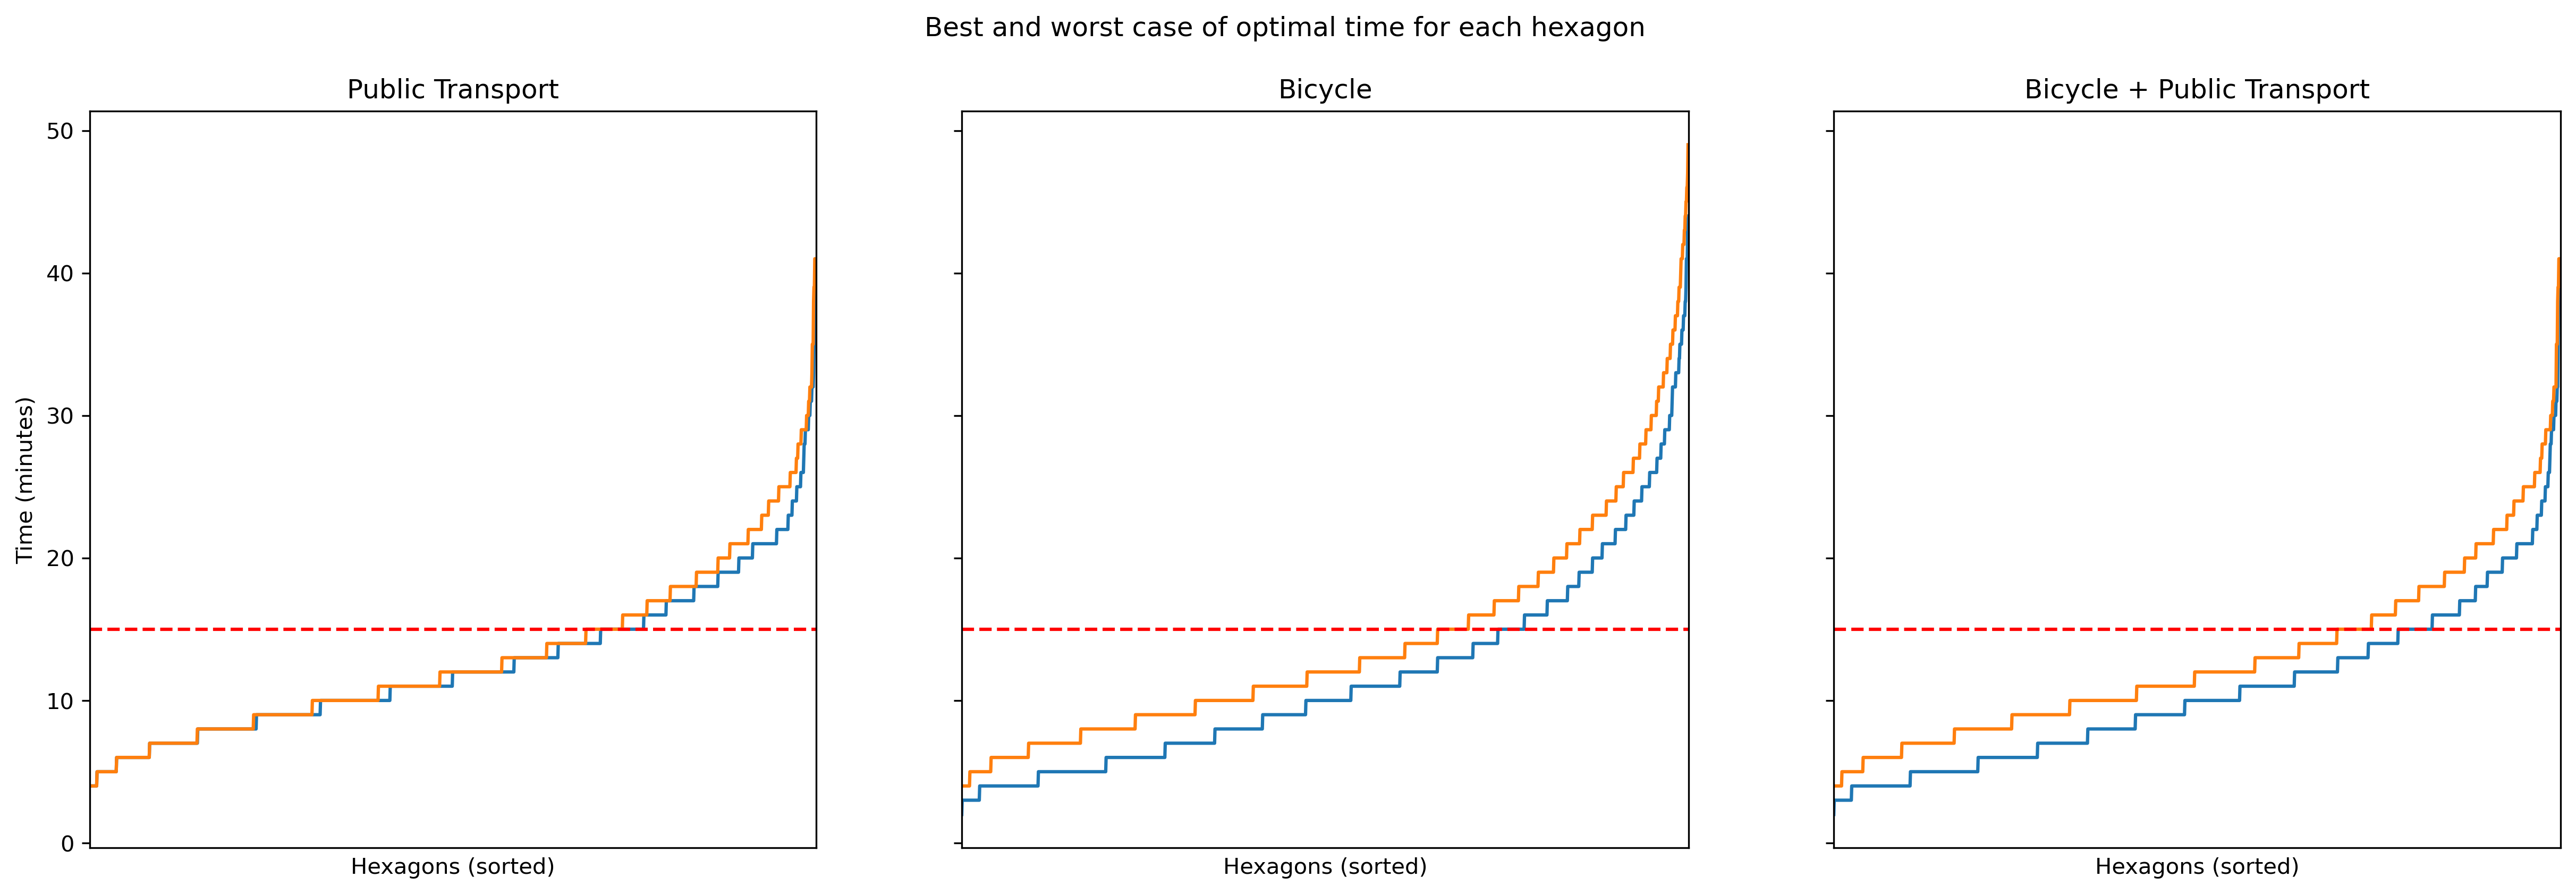
\includegraphics[width=0.95\textwidth]{Figures/results/uncertainty/optimal_best_worst_case}
  \end{center}
  \caption{Best and Worst Case of Optimal Time for each Hexagon}
  \label{fig:best_and_worst_case_of_optimal_time_for_each_hexagon}
\end{figure}
First, we see that the variation for bicycles is spread out over almost all hexagons, in comparison to public transport where the variation only really begins to happen after the 15-minute mark.
For the combined scenario, we see the expected: The variances of the public transport scenario and the bicycle scenario add up.

\subsection{Impact Of Sustainable Modes on 15-Minute Metric}
\label{subsec:impact_of_sustainable_modes_on_15_minute_metric}

To analyze the impact of sustainable modes of travel on the 15-minute city metric, we first uncover the problematic areas in which the X-minute city metric is above 15 minutes for the walking mode.
We then analyze how sustainable modes of travel can help reduce the X-minute city metric in those areas below 15 minutes.

In total, we find 552 hexagons with a walking time of more than 15 minutes to reach all POI categories, which is 30.98\% of all hexagons.
\begin{table}[h]
  \centering
  \begin{tabular}{|l|l|}
    \hline
    \textbf{Category}                                          & \textbf{Data}                \\ \hline
    Only bicycle below 15 mins                                 & 72 (13.04\%)                 \\ \hline
    Only public transport below 15 mins                        & 59 (10.69\%)                 \\ \hline
    Both bicycle and public transport below 15 mins            & 41 (7.43\%)                  \\ \hline
    Combined mode below 15 mins                                & 10 (1.81\%)                  \\ \hline
    Not reachable by sustainable modes below 15 mins           & 370 (67.03\%)                \\ \hline
  \end{tabular}
  \caption{Impact of Sustainable Modes on Reducing Walking Time Above 15 Minutes}
  \label{table:hexagons_with_walking_time_above_15_minutes}
\end{table}
Table \ref{table:hexagons_with_walking_time_above_15_minutes} presents the distribution of hexagons with a walking time above 15 minutes and how sustainable modes of transport can fix those hexagons.
By fixing a hexagon, we mean that residents in the hexagon cannot reach all necessities in under 15 minutes by walking, but they can make it in under 15 minutes by some other mode of transport.
A significant portion of these areas, amounting to 67.03\%, cannot be reached within 15 minutes using sustainable modes with the current state of infrastructure. 
Conversely, the data indicates that for 13.04\% of these hexagons, only bicycles can reduce travel time to under 15 minutes, while only public transport can achieve this for 10.69\% of the hexagons. 
7.43\% of hexagons are reachable with either one of bicycles or public transport, while an additional 1.81\% of hexagons are only accessible within this time frame when combining both modes. 


Next, we visualize these problematic areas spatially.
Figure \ref{fig:problematic_hexagons} displays hexagons in green where necessities can be reached within a 15-minute walk, in yellow where they are only accessible within 15 minutes using any sustainable transport, and in red where necessities are not reachable within this 15-minute timeframe.
\begin{figure}
  \begin{center}
    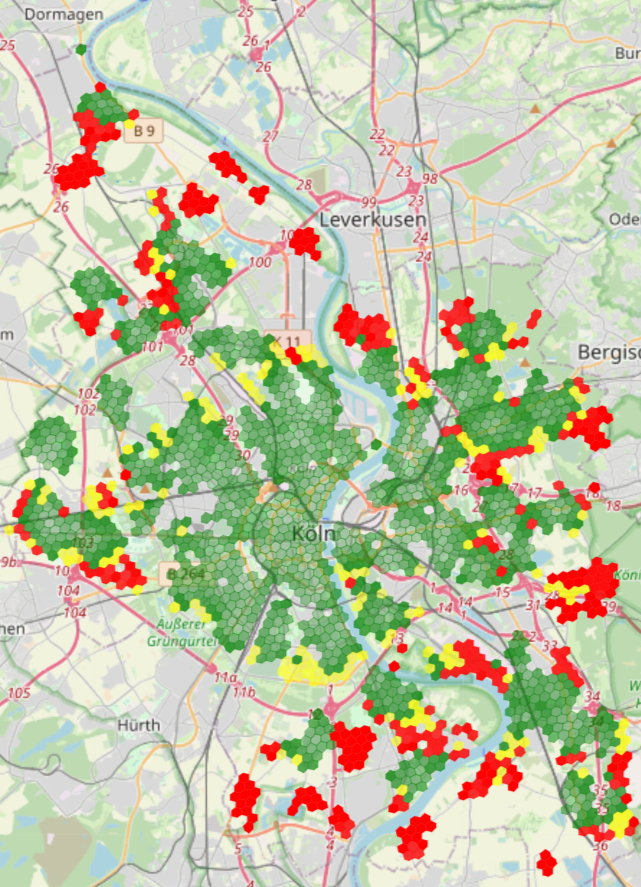
\includegraphics[width=0.50\textwidth]{Figures/results/problematic_hexagons/problematic_hexagons}
  \end{center}
  \caption{Unfixable, Fixable and Unproblematic Hexagons on a Map}
  \label{fig:problematic_hexagons}
\end{figure}
We see that in the center of Cologne, almost all hexagons qualify as 15-minute city hexagons just by walking alone.
At the city's border, we see a ring of hexagons that are only valid 15-minute hexagons through additional modes of transport.
Most of the unfixable hexagons lie in the city's suburbs, often appearing in larger groups.

Next, we look at the hexagons previously colored yellow, namely those where bicycles and public transport or a combination of both can decrease the 15-minute city metric below 15 minutes.
Figure \ref{fig:fixable_hexagons} illustrates hexagons representing areas that qualify as 15-minute cities via public transport in yellow, those that qualify through bicycle sharing in orange, and areas that meet the 15-minute city criteria through either mode in green.
\begin{figure}
  \begin{center}
    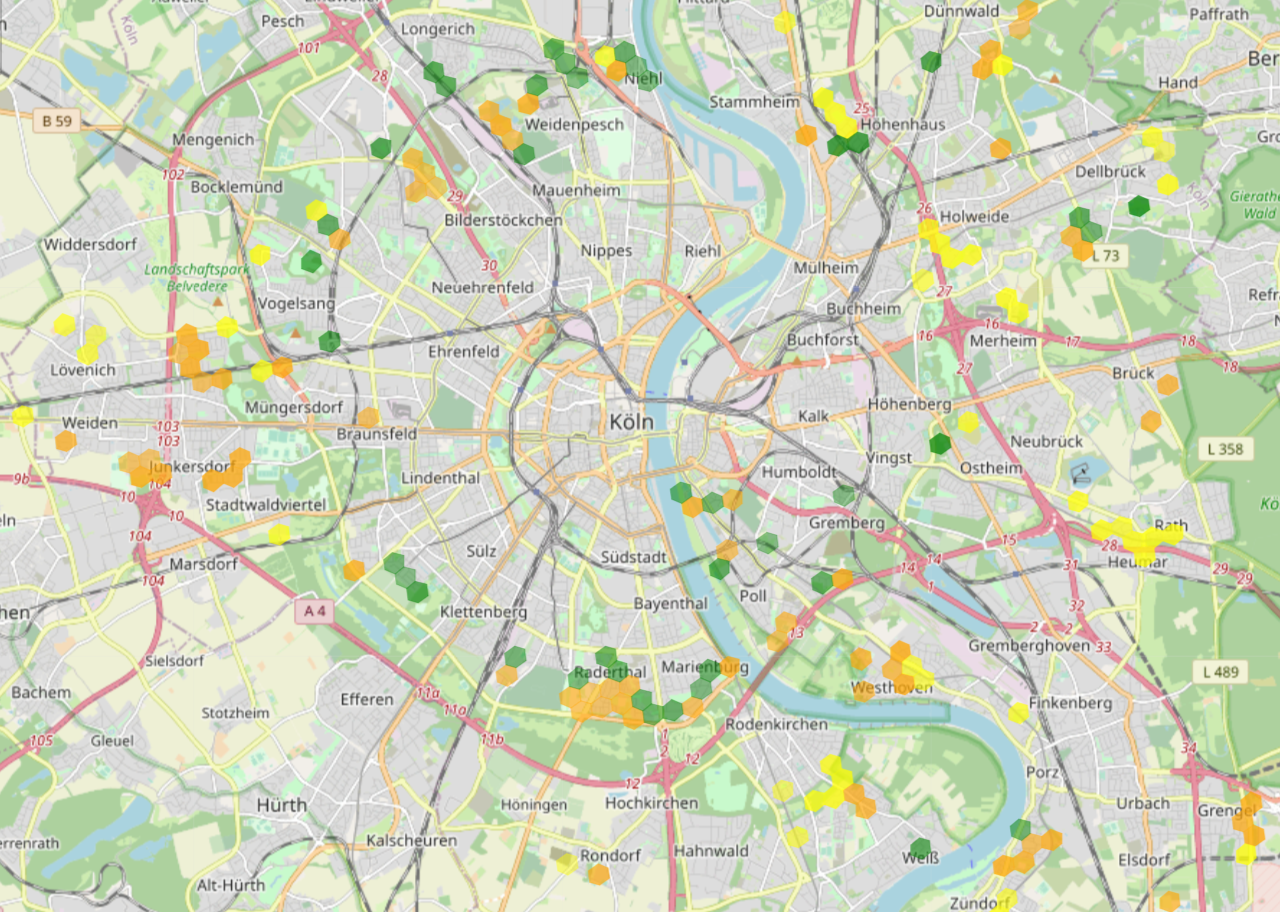
\includegraphics[width=0.70\textwidth]{Figures/results/problematic_hexagons/fixable_hexagons}
  \end{center}
  \caption{Fixable Hexagons by Mode}
  \label{fig:fixable_hexagons}
\end{figure}
The data indicates a modest trend where hexagons that achieve 15-minute city criteria solely through bicycle sharing (marked in orange) tend to be nearer to the city center than those that achieve this criterion solely via public transport.

The positions of outer clusters of fixable hexagons correlate directly with the locations of bicycles and public transport stops.
Figure \ref{fig:fixable_hexagons_examples} shows four zoomed-in excerpts from Figure \ref{fig:fixable_hexagons}, where we've added the location of public transport stops and bicycles.
\begin{figure}
     \centering
     \begin{subfigure}[b]{0.45\textwidth}
         \centering
         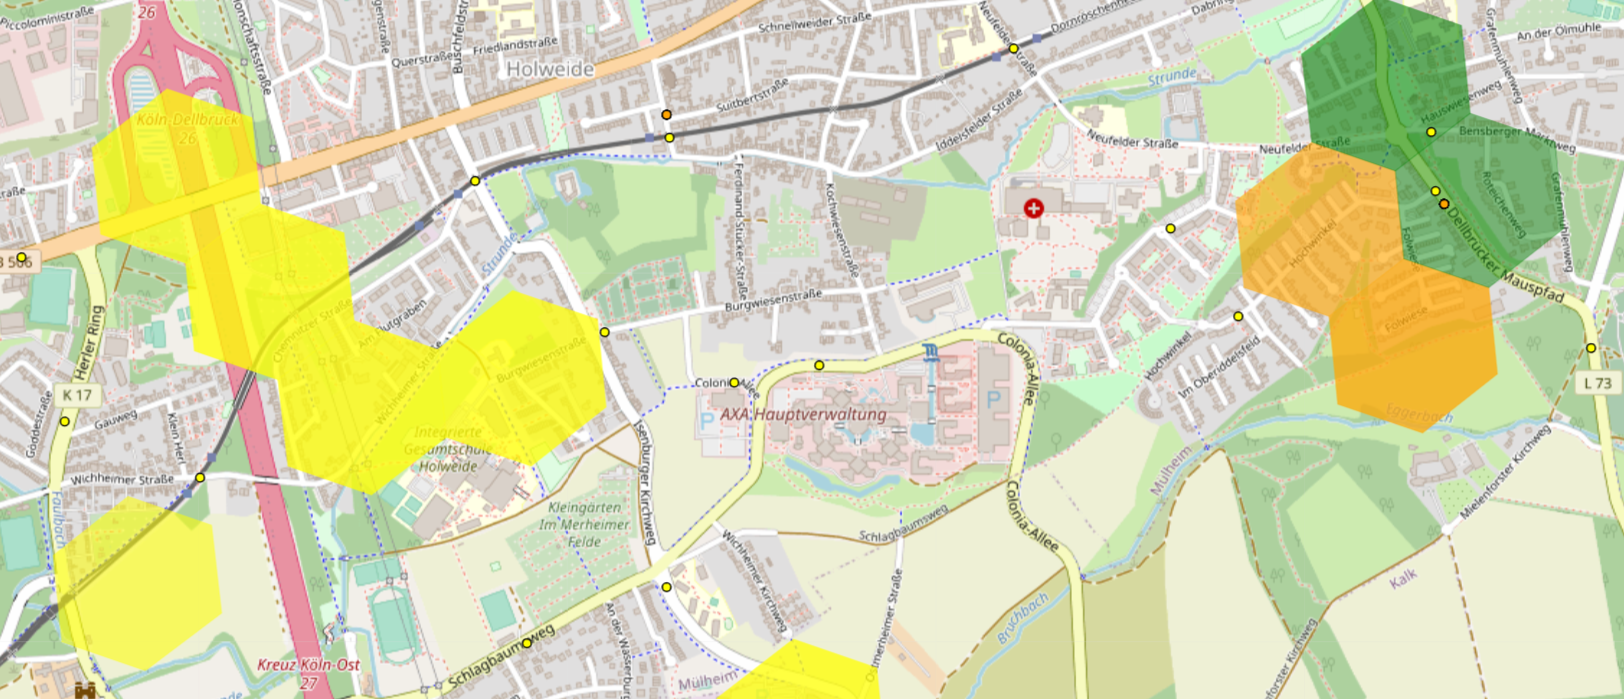
\includegraphics[width=\textwidth]{Figures/results/problematic_hexagons/example_1.png}
     \end{subfigure}
     \hfill
     \begin{subfigure}[b]{0.45\textwidth}
         \centering
         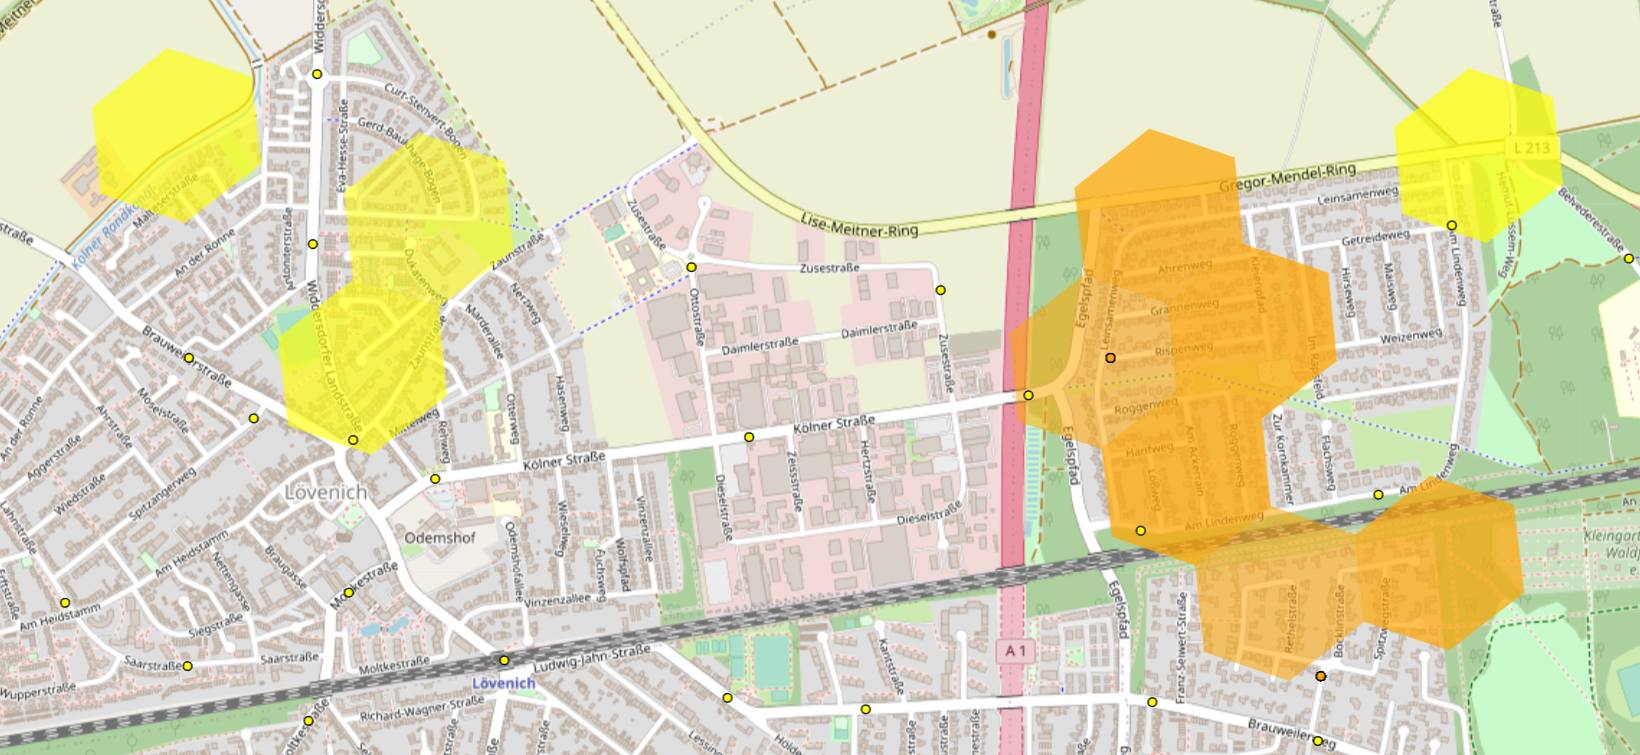
\includegraphics[width=\textwidth]{Figures/results/problematic_hexagons/example_2.png}
     \end{subfigure}
     \hfill
     \begin{subfigure}[b]{0.45\textwidth}
         \centering
         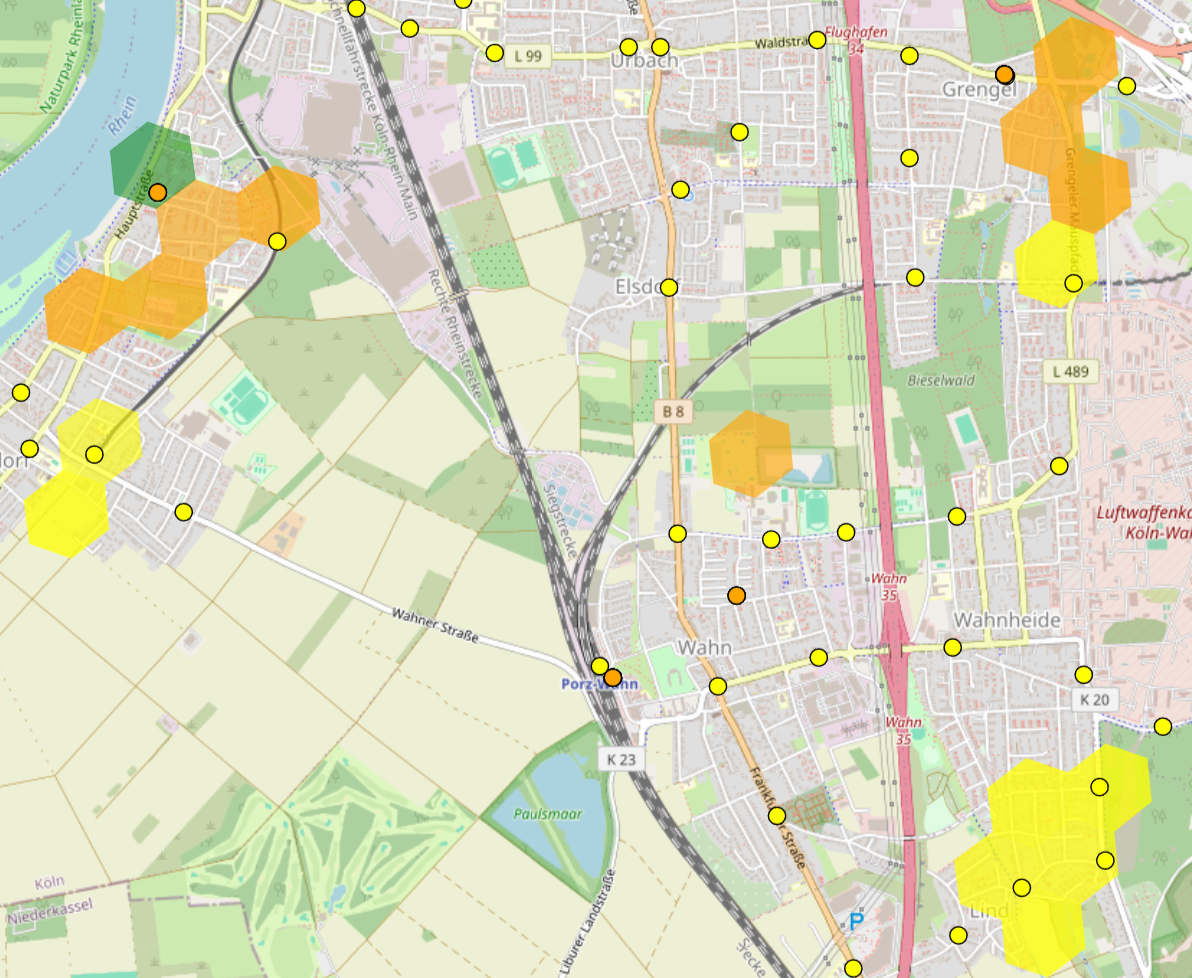
\includegraphics[width=\textwidth]{Figures/results/problematic_hexagons/example_3.png}
     \end{subfigure}
     \hfill
     \begin{subfigure}[b]{0.45\textwidth}
         \centering
         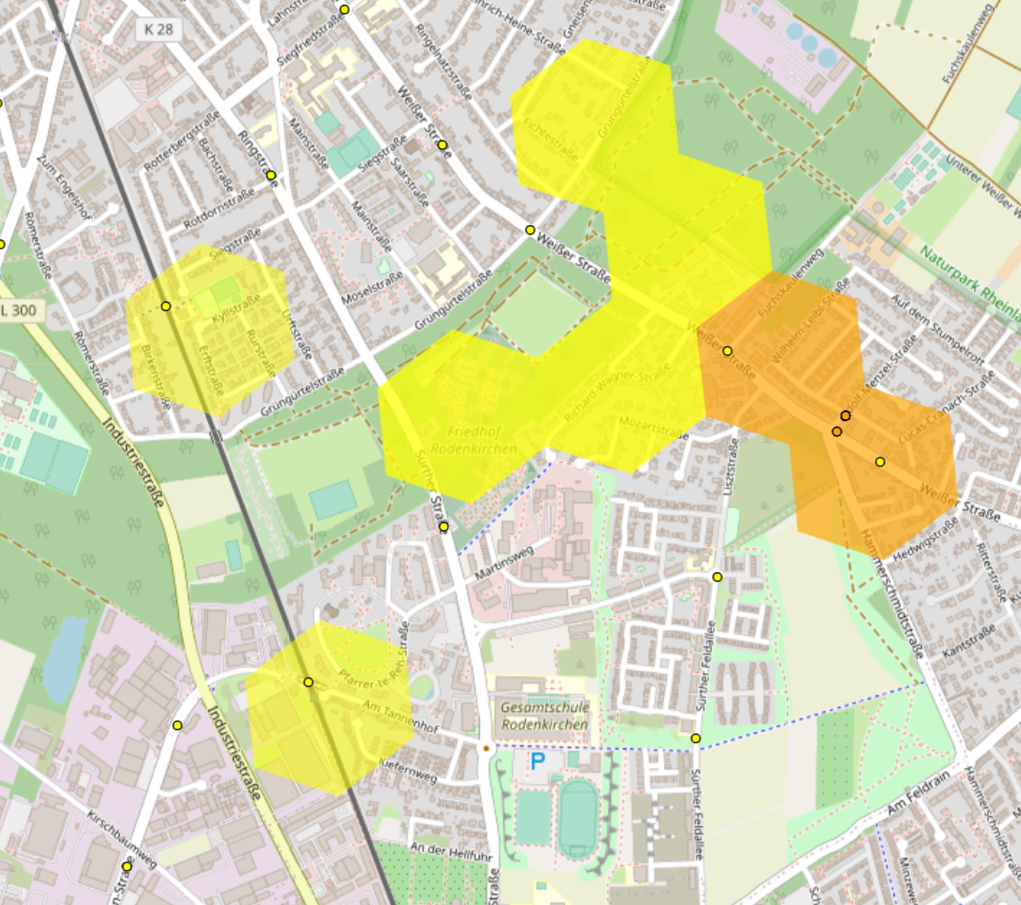
\includegraphics[width=\textwidth]{Figures/results/problematic_hexagons/example_4.png}
     \end{subfigure}
     \caption{Examples of Fixable Hexagons}
        \label{fig:fixable_hexagons_examples}
\end{figure}
Public transport stops are visualized as yellow circles, while bicycles are visualized as orange circles.
We notice that hexagons fixed by bicycle sharing are always near bicycles.
In the same way, hexagons fixed better by public transport are always close to public transport stops. 
However, being close to bike stations seems to have a more significant effect than being near public transport stops.

Figure \ref{fig:only_unfixable_hexagons} shows all hexagons that are not 15-minute hexagons by any sustainable mode of transport.
Figure \ref{fig:unfixable_with_bicycles} and \ref{fig:unfixable_with_stops} show the same map but with additional bicycle locations and public transport stop locations, respectively.
\begin{figure}
     \centering
     \begin{subfigure}[b]{0.30\textwidth}
         \centering
         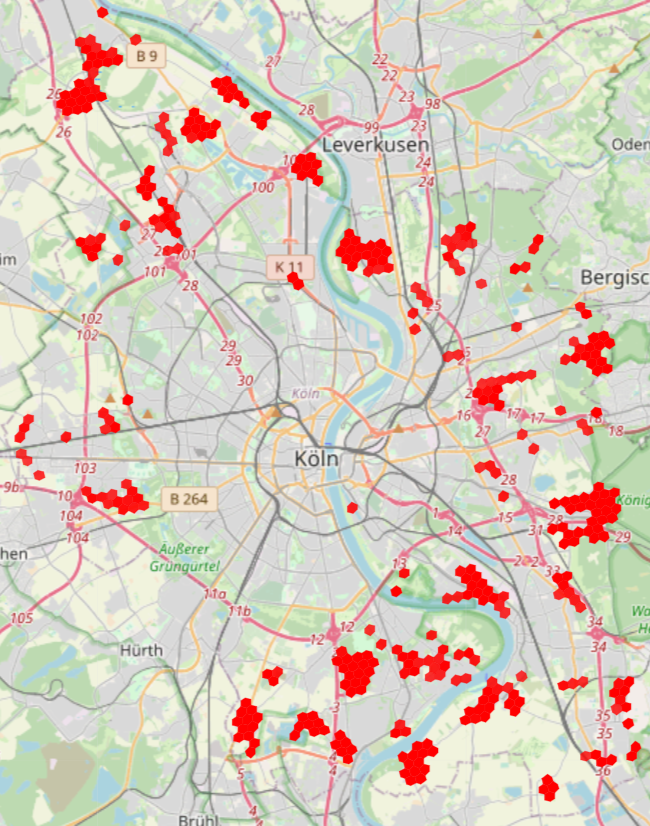
\includegraphics[width=\textwidth]{Figures/results/problematic_hexagons/unfixable.png}
         \caption{Only Unfixable Hexagons}
         \label{fig:only_unfixable_hexagons}
     \end{subfigure}
     \hfill
     \begin{subfigure}[b]{0.30\textwidth}
         \centering
         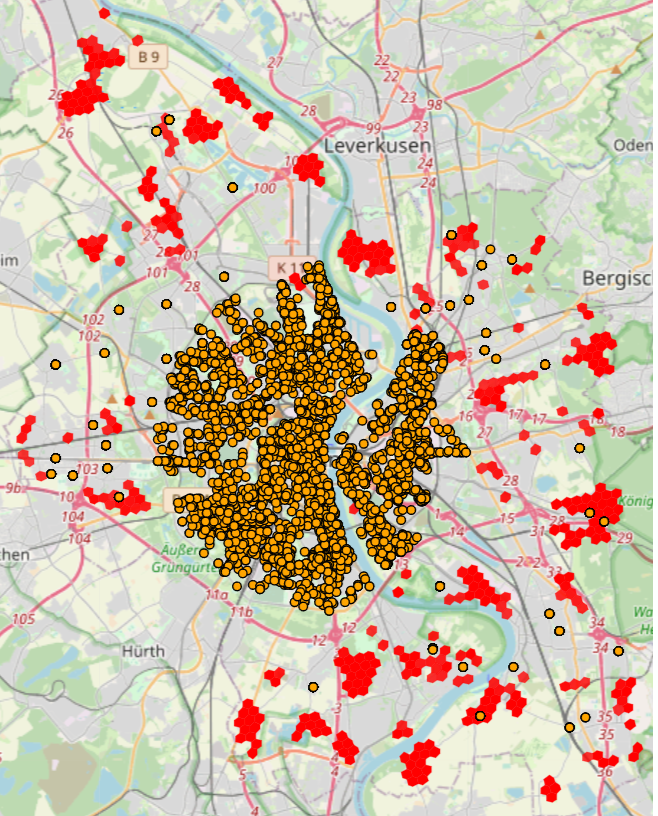
\includegraphics[width=\textwidth]{Figures/results/problematic_hexagons/unfixable_with_bicycles.png}
         \caption{With All Bicycle Locations}
         \label{fig:unfixable_with_bicycles}
     \end{subfigure}
     \hfill
     \begin{subfigure}[b]{0.30\textwidth}
         \centering
         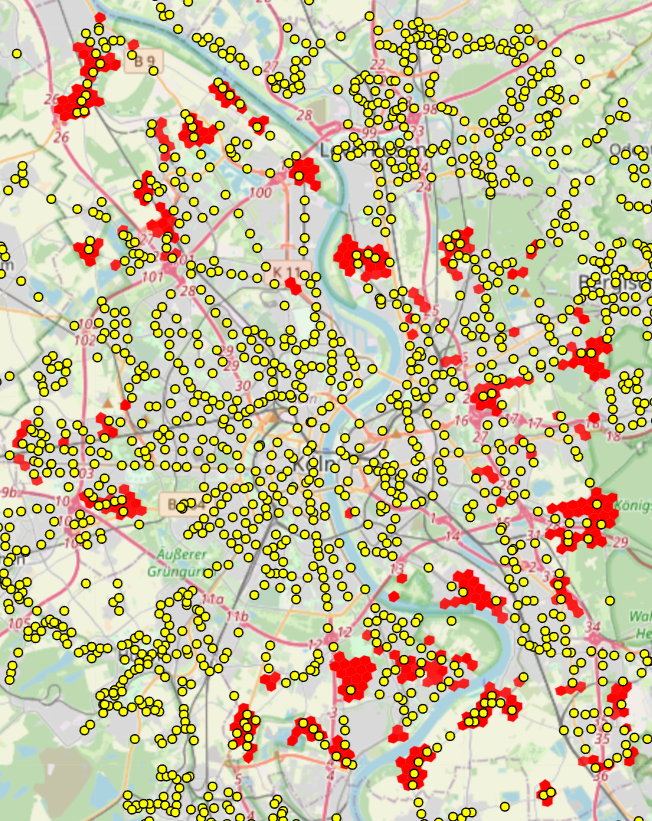
\includegraphics[width=\textwidth]{Figures/results/problematic_hexagons/unfixable_with_stops.png}
         \caption{With Public Transport Stops}
         \label{fig:unfixable_with_stops}
     \end{subfigure}
     \hfill
     \caption{Unfixable Hexagons}
     \label{fig:unfixable_hexagons}
\end{figure}
We can observe that the unfixable hexagons mostly do not contain any bicycles and have a larger distance to the nearest bicycle.
The same cannot be said for public transport stops, as public transport stops are often directly inside the unfixable hexagons.

Figure \ref{fig:combined_hexagons} shows all hexagons that only become 15-minute city hexagons in the combined scenario when public transport and bicycle sharing are used simultaneously.
As already seen in Table \ref{table:hexagons_with_walking_time_above_15_minutes}, this only concerns less than 2\% of all hexagons that are not already 15-minute city hexagons through walking alone.
More than half of those (7 out of 10) are located in the southern district of Weiß.
\begin{figure}
  \begin{center}
    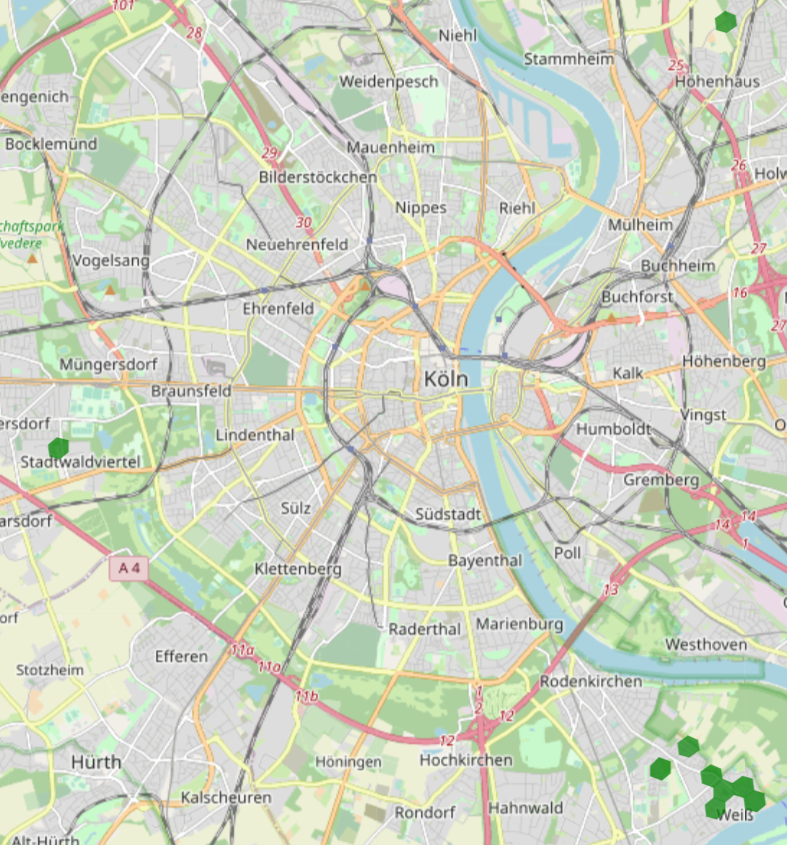
\includegraphics[width=0.50\textwidth]{Figures/results/problematic_hexagons/combined_hexagons}
  \end{center}
  \caption{Hexagons Fixable by Combined Mode}
  \label{fig:combined_hexagons}
\end{figure}


\subsection{Monthly Costs Per Scenario And Hexagon}
\label{sec:monthly_costs}
A prevalent measure to incentivize sustainable modes of transport are monthly tickets or subscriptions.
To measure whether the costs of these subscriptions are worth it, we will calculate the monthly cost incurred by the trips to all necessities.
To do so, we first collect how often people visit each POI category we defined earlier.
Table \ref{tab:monthly_visits} shows the monthly number of visits per category we've collected from various sources.
The derivation of these numbers, as well as, the sources can be found in Appendix \ref{app:monthly_visits_per_category}

To understand and compare the usual monthly costs caused by traveling with different modes of transport, we first establish two time-based benchmarks to compare the cost incurred.
The first benchmark focuses on the costs incurred when reaching the nearest POI of a given category within a 15-minute timeframe. 
The second benchmark assesses the costs for a similar journey but within a more constrained 10-minute limit.
However, to compare these costs, a journey in that time has to be possible, which is not always the case.

\begin{table}
  \caption{Number of Monthly Visits per Category}
  \label{tab:monthly_visits}
  \begin{center}
    \begin{tabular}[c]{l|l}
      category & monthly visits \\
      \hline
      groceries & 12 \\
      education & 20 \\
      health & 0.42 \\
      banks & 9 \\
      parks & 2.4 \\
      sustenance & 6.12 \\
      shops & 4 \\
      \hline
    \end{tabular}
  \end{center}
\end{table}

Therefore, we show how often a journey is possible within the given timeframe in Figure \ref{fig:percentage_inf_x}.
In the 10-minute benchmark, the combined scenario of bicycle sharing and public transport fails the least, with a maximum of 36\% for the bank category, followed by public transport and bicycle sharing.
In the 15-minute benchmark, bicycle sharing and public transport perform almost equally well, while in the 10-minute benchmark, bicycle sharing performs better than public transport.
Category-wise, banks seem to be the least accessible category, followed by parks and health.
Sustenance, education, grocery, and shops all seem similarly accessible.

\begin{figure}
  \centering
  \begin{subfigure}[b]{0.45\textwidth}
    \centering
    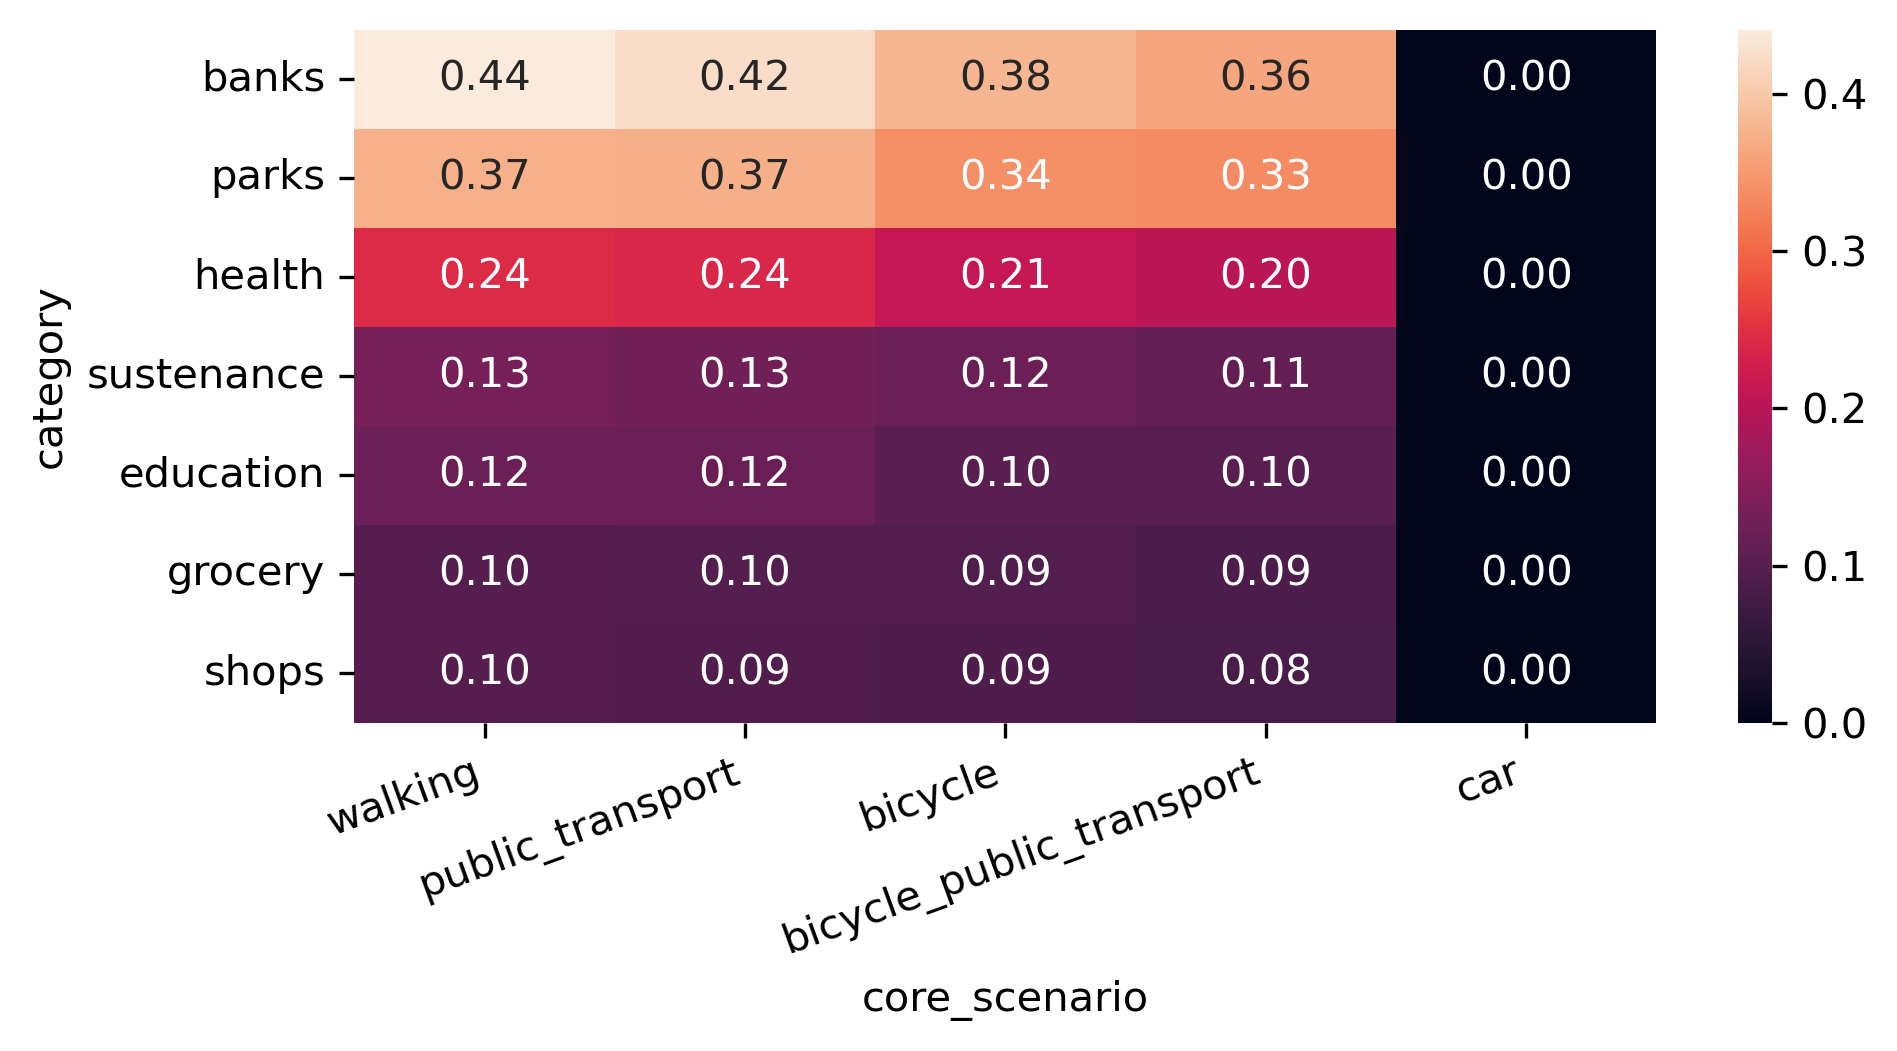
\includegraphics[width=\textwidth]{Figures/results/monthly_costs/percentage_inf_10.png}
    \caption{10 Minutes}
    \label{fig:percentage_inf_10}
  \end{subfigure}
  \hfill
  \begin{subfigure}[b]{0.45\textwidth}
    \centering
    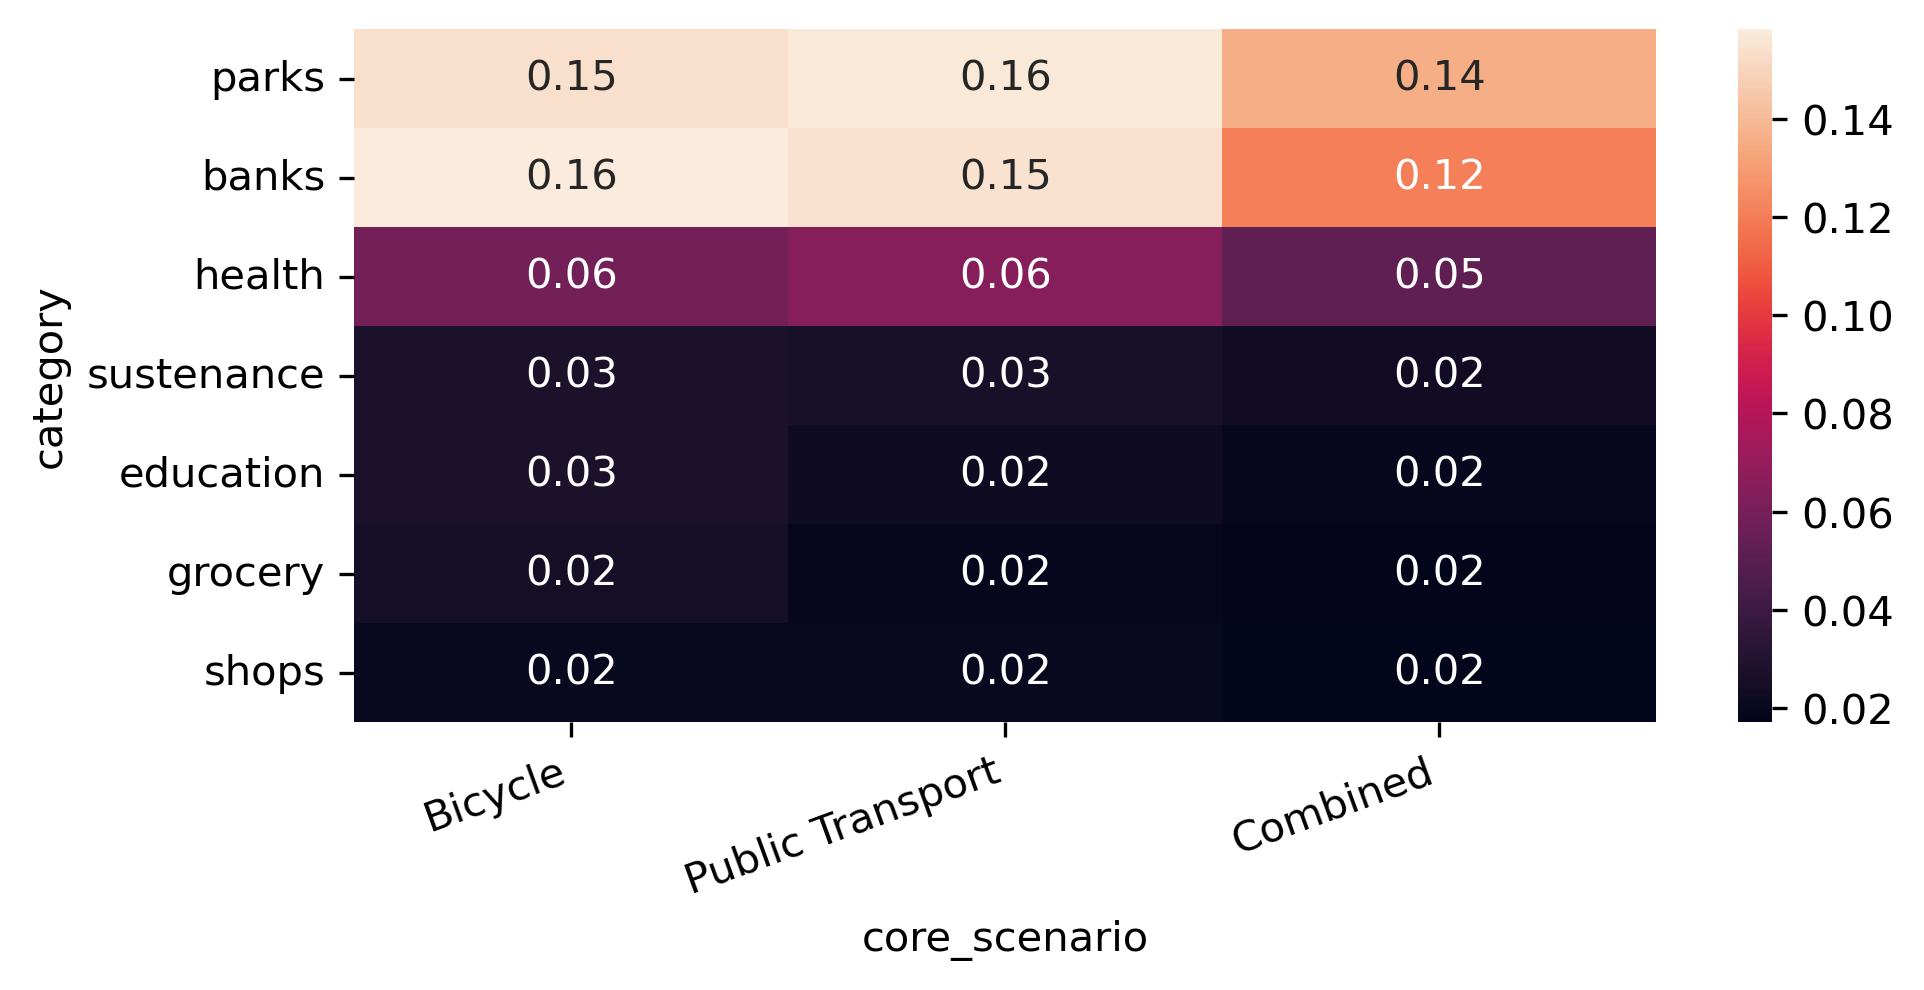
\includegraphics[width=\textwidth]{Figures/results/monthly_costs/percentage_inf_15.png}
    \caption{15 Minutes}
    \label{fig:percentage_inf_15}
  \end{subfigure}
  \caption{Impossible Sub-X-Minute Journeys for each Hexagon and Scenario}
  \label{fig:percentage_inf_x}
\end{figure}

As seen in the previously discussed Figure \ref{fig:percentage_inf_x}, the number of impossible journeys differs across scenarios.
This, again, makes it hard to compare the costs across scenarios.
Therefore, we will only look at hexagons and category combinations where a journey is possible within the given timeframe for all scenarios with sustainable transport modes.
In addition, we also filter out hexagon category combinations where the cost is zero, i.e. where walking suffices, as those are not interesting for our cost analysis.

\begin{table}
  \caption{Monthly costs per scenario (<15 minutes)}
  \label{tab:monthly_costs_per_scenario_15}
  \begin{center}
    \begin{tabular}{lrrrrrrr}
     & mean & std & min & 25\% & 50\% & 75\% & max \\
    Scenario &  &  &  &  &  &  &  \\
    Bicycle & 5.79 & 5.95 & 0.42 & 0.42 & 4.00 & 9.00 & 29.00 \\
    Combined & 5.79 & 5.95 & 0.42 & 0.42 & 4.00 & 9.00 & 29.00 \\
    Public Transport & 12.93 & 13.26 & 0.93 & 0.93 & 8.80 & 19.80 & 63.80 \\
    \end{tabular}
  \end{center}
\end{table}


\begin{table}
  \caption{Monthly costs per scenario (<10 minutes)}
  \label{tab:monthly_costs_per_scenario_10}
  \begin{center}
    \begin{tabular}{lrrrrrrr}
     & mean & std & min & 25\% & 50\% & 75\% & max \\
    Scenario &  &  &  &  &  &  &  \\
    Bicycle & 10.49 & 7.72 & 0.42 & 2.42 & 9.00 & 20.00 & 24.54 \\
    Combined & 10.49 & 7.72 & 0.42 & 2.42 & 9.00 & 20.00 & 24.54 \\
    Public Transport & 23.08 & 16.98 & 0.93 & 5.32 & 19.80 & 44.00 & 53.98 \\
    \end{tabular}
  \end{center}
\end{table}

Table \ref{tab:monthly_costs_per_scenario_15} shows the average monthly costs to reach all categories within 15 minutes for each scenario, and Table \ref{tab:monthly_costs_per_scenario_10} shows the same for 10 minutes.
As we can see, the total cost averages at \euro{5.80} for the bicycle and combined scenario and \euro{12.90} for the public transport scenario in the 15-minute benchmark.
The cost reaches a maximum of \euro{29} for the bicycle and combined scenario and \euro{63.8} for the public transport scenario, while the 25\% most expensive hexagons require residents to pay at least \euro{9} for the bicycle and combined scenario and \euro{19.80} for the public transport scenario.
Note that the bicycle and combined scenario always have the same cost, showing that it is not worth to use public transport, when bicycle sharing is available in those hexagons.
In the 10-minute benchmark, the average cost is \euro{10.5} for the bicycle and combined scenario and \euro{23.1} for the public transport scenario.
Here, the cost reaches a maximum of \euro{24.54} for the bicycle and combined scenario and \euro{53.98} for the public transport scenario, while the 25\% most expensive hexagons require residents to pay at least \euro{20} for the bicycle and combined scenario and \euro{44} for the public transport scenario.

\begin{table}
  \caption{Monthly costs for cars}
  \label{tab:monthly_costs_for_cars}
  \begin{center}
    \begin{tabular}{lrrrrrrr}
     & mean & std & min & 25\% & 50\% & 75\% & max \\
    Car (15 Minutes) & 1.79 & 1.69 & 0.00 & 0.46 & 1.71 & 1.79 & 7.00 \\
    Car (10 Minutes) & 2.87 & 2.89 & 0.00 & 0.46 & 1.79 & 3.91 & 10.88 \\
    \end{tabular}
  \end{center}
\end{table}

Next, we will also look at the monthly costs for the car scenario in the same hexagons we considered previously in Figure \ref{tab:monthly_costs_for_cars}.
This allows us to compare the cost of cars with other modes of transport.
We see that the average cost is \euro{1.79} for the 15-minute benchmark and \euro{2.87} for the 10-minute benchmark, which in both cases is less than a third of the cheapest sustainable mode of transport.
However, remember that the cost of \euro{0.19}/min tries to capture fuel costs, repair costs, insurance, and tax, but not acquisition costs.
